\documentclass[twoside]{book}

% Packages required by doxygen
\usepackage{calc}
\usepackage{doxygen}
\usepackage{graphicx}
\usepackage[utf8]{inputenc}
\usepackage{makeidx}
\usepackage{multicol}
\usepackage{multirow}
\usepackage{textcomp}
\usepackage[table]{xcolor}

% NLS support packages
\usepackage[spanish]{babel}
% Font selection
\usepackage[T1]{fontenc}
\usepackage{mathptmx}
\usepackage[scaled=.90]{helvet}
\usepackage{courier}
\usepackage{amssymb}
\usepackage{sectsty}
\renewcommand{\familydefault}{\sfdefault}
\allsectionsfont{%
  \fontseries{bc}\selectfont%
  \color{darkgray}%
}
\renewcommand{\DoxyLabelFont}{%
  \fontseries{bc}\selectfont%
  \color{darkgray}%
}

% Page & text layout
\usepackage{geometry}
\geometry{%
  a4paper,%
  top=2.5cm,%
  bottom=2.5cm,%
  left=2.5cm,%
  right=2.5cm%
}
\tolerance=750
\hfuzz=15pt
\hbadness=750
\setlength{\emergencystretch}{15pt}
\setlength{\parindent}{0cm}
\setlength{\parskip}{0.2cm}
\makeatletter
\renewcommand{\paragraph}{%
  \@startsection{paragraph}{4}{0ex}{-1.0ex}{1.0ex}{%
    \normalfont\normalsize\bfseries\SS@parafont%
  }%
}
\renewcommand{\subparagraph}{%
  \@startsection{subparagraph}{5}{0ex}{-1.0ex}{1.0ex}{%
    \normalfont\normalsize\bfseries\SS@subparafont%
  }%
}
\makeatother

% Headers & footers
\usepackage{fancyhdr}
\pagestyle{fancyplain}
\fancyhead[LE]{\fancyplain{}{\bfseries\thepage}}
\fancyhead[CE]{\fancyplain{}{}}
\fancyhead[RE]{\fancyplain{}{\bfseries\leftmark}}
\fancyhead[LO]{\fancyplain{}{\bfseries\rightmark}}
\fancyhead[CO]{\fancyplain{}{}}
\fancyhead[RO]{\fancyplain{}{\bfseries\thepage}}
\fancyfoot[LE]{\fancyplain{}{}}
\fancyfoot[CE]{\fancyplain{}{}}
\fancyfoot[RE]{\fancyplain{}{\bfseries\scriptsize Generado el Martes, 1 de Abril de 2014 09\-:10\-:54 para /home/linuxero/\-Net\-Beans\-Projects/prueba\-\_\-colisiones por Doxygen }}
\fancyfoot[LO]{\fancyplain{}{\bfseries\scriptsize Generado el Martes, 1 de Abril de 2014 09\-:10\-:54 para /home/linuxero/\-Net\-Beans\-Projects/prueba\-\_\-colisiones por Doxygen }}
\fancyfoot[CO]{\fancyplain{}{}}
\fancyfoot[RO]{\fancyplain{}{}}
\renewcommand{\footrulewidth}{0.4pt}
\renewcommand{\chaptermark}[1]{%
  \markboth{#1}{}%
}
\renewcommand{\sectionmark}[1]{%
  \markright{\thesection\ #1}%
}

% Indices & bibliography
\usepackage{natbib}
\usepackage[titles]{tocloft}
\setcounter{tocdepth}{3}
\setcounter{secnumdepth}{5}
\makeindex

% Hyperlinks (required, but should be loaded last)
\usepackage{ifpdf}
\ifpdf
  \usepackage[pdftex,pagebackref=true]{hyperref}
\else
  \usepackage[ps2pdf,pagebackref=true]{hyperref}
\fi
\hypersetup{%
  colorlinks=true,%
  linkcolor=blue,%
  citecolor=blue,%
  unicode%
}

% Custom commands
\newcommand{\clearemptydoublepage}{%
  \newpage{\pagestyle{empty}\cleardoublepage}%
}


%===== C O N T E N T S =====

\begin{document}

% Titlepage & ToC
\hypersetup{pageanchor=false}
\pagenumbering{roman}
\begin{titlepage}
\vspace*{7cm}
\begin{center}%
{\Large /home/linuxero/\-Net\-Beans\-Projects/prueba\-\_\-colisiones }\\
\vspace*{1cm}
{\large Generado por Doxygen 1.8.6}\\
\vspace*{0.5cm}
{\small Martes, 1 de Abril de 2014 09:10:54}\\
\end{center}
\end{titlepage}
\clearemptydoublepage
\tableofcontents
\clearemptydoublepage
\pagenumbering{arabic}
\hypersetup{pageanchor=true}

%--- Begin generated contents ---
\chapter{Arquitectura con Colisiones, Movimientos y Físicas}
\label{md__home_linuxero_NetBeansProjects_prueba_colisiones_README}
\hypertarget{md__home_linuxero_NetBeansProjects_prueba_colisiones_README}{}
Ejecutable donde, mediante una mini-\/\-Arquitectura de videojuego, se prueban las Colisiones, Movimientos y Físicas.

Se puede encontrar documentación en la carpeta {\bfseries doc/} 
\chapter{Indice jerárquico}
\section{Jerarquía de la clase}
Esta lista de herencias esta ordenada aproximadamente por orden alfabético\-:\begin{DoxyCompactList}
\item \contentsline{section}{Clock}{\pageref{classClock}}{}
\item \contentsline{section}{Colisionable}{\pageref{classColisionable}}{}
\begin{DoxyCompactList}
\item \contentsline{section}{Bullet}{\pageref{classBullet}}{}
\item \contentsline{section}{Enemy}{\pageref{classEnemy}}{}
\item \contentsline{section}{Player}{\pageref{classPlayer}}{}
\end{DoxyCompactList}
\item \contentsline{section}{Entity}{\pageref{classEntity}}{}
\begin{DoxyCompactList}
\item \contentsline{section}{Ent\-Active}{\pageref{classEntActive}}{}
\begin{DoxyCompactList}
\item \contentsline{section}{Bullet}{\pageref{classBullet}}{}
\item \contentsline{section}{Enemy}{\pageref{classEnemy}}{}
\item \contentsline{section}{Gun}{\pageref{classGun}}{}
\item \contentsline{section}{Player}{\pageref{classPlayer}}{}
\end{DoxyCompactList}
\item \contentsline{section}{Ent\-Passive}{\pageref{classEntPassive}}{}
\end{DoxyCompactList}
\item \contentsline{section}{Level}{\pageref{classLevel}}{}
\item \contentsline{section}{Maths}{\pageref{classMaths}}{}
\item \contentsline{section}{Physics\-State}{\pageref{classPhysicsState}}{}
\item \contentsline{section}{Rectangle}{\pageref{classRectangle}}{}
\item \contentsline{section}{Render\-State}{\pageref{classRenderState}}{}
\item \contentsline{section}{Render\-Window}{\pageref{classRenderWindow}}{}
\item \contentsline{section}{Resource\-Holder$<$ Resource, Identifier $>$}{\pageref{classResourceHolder}}{}
\item \contentsline{section}{Resource\-Holder$<$ sf\-:\-:Font, std\-:\-:string $>$}{\pageref{classResourceHolder}}{}
\item \contentsline{section}{Resource\-Holder$<$ sf\-:\-:Texture, std\-:\-:string $>$}{\pageref{classResourceHolder}}{}
\item \contentsline{section}{Singleton}{\pageref{classSingleton}}{}
\item \contentsline{section}{Sprite}{\pageref{classSprite}}{}
\item \contentsline{section}{String\-Utils}{\pageref{classStringUtils}}{}
\item \contentsline{section}{Time}{\pageref{classTime}}{}
\item \contentsline{section}{Vector}{\pageref{classVector}}{}
\item \contentsline{section}{World}{\pageref{classWorld}}{}
\end{DoxyCompactList}

\chapter{Índice de clases}
\section{Lista de clases}
Lista de las clases, estructuras, uniones e interfaces con una breve descripción\-:\begin{DoxyCompactList}
\item\contentsline{section}{\hyperlink{classBullet}{Bullet} }{\pageref{classBullet}}{}
\item\contentsline{section}{\hyperlink{classClock}{Clock} }{\pageref{classClock}}{}
\item\contentsline{section}{\hyperlink{classColisionable}{Colisionable} }{\pageref{classColisionable}}{}
\item\contentsline{section}{\hyperlink{classEnemy}{Enemy} }{\pageref{classEnemy}}{}
\item\contentsline{section}{\hyperlink{classEntActive}{Ent\-Active} }{\pageref{classEntActive}}{}
\item\contentsline{section}{\hyperlink{classEntity}{Entity} }{\pageref{classEntity}}{}
\item\contentsline{section}{\hyperlink{classEntPassive}{Ent\-Passive} }{\pageref{classEntPassive}}{}
\item\contentsline{section}{\hyperlink{classGun}{Gun} }{\pageref{classGun}}{}
\item\contentsline{section}{\hyperlink{classLevel}{Level} }{\pageref{classLevel}}{}
\item\contentsline{section}{\hyperlink{classMaths}{Maths} }{\pageref{classMaths}}{}
\item\contentsline{section}{\hyperlink{classPhysicsState}{Physics\-State} }{\pageref{classPhysicsState}}{}
\item\contentsline{section}{\hyperlink{classPlayer}{Player} }{\pageref{classPlayer}}{}
\item\contentsline{section}{\hyperlink{classRectangle}{Rectangle} }{\pageref{classRectangle}}{}
\item\contentsline{section}{\hyperlink{classRenderState}{Render\-State} }{\pageref{classRenderState}}{}
\item\contentsline{section}{\hyperlink{classRenderWindow}{Render\-Window} }{\pageref{classRenderWindow}}{}
\item\contentsline{section}{\hyperlink{classResourceHolder}{Resource\-Holder$<$ Resource, Identifier $>$} }{\pageref{classResourceHolder}}{}
\item\contentsline{section}{\hyperlink{classSingleton}{Singleton} }{\pageref{classSingleton}}{}
\item\contentsline{section}{\hyperlink{classSprite}{Sprite} }{\pageref{classSprite}}{}
\item\contentsline{section}{\hyperlink{classStringUtils}{String\-Utils} }{\pageref{classStringUtils}}{}
\item\contentsline{section}{\hyperlink{classTime}{Time} }{\pageref{classTime}}{}
\item\contentsline{section}{\hyperlink{classVector}{Vector} }{\pageref{classVector}}{}
\item\contentsline{section}{\hyperlink{classWorld}{World} }{\pageref{classWorld}}{}
\end{DoxyCompactList}

\chapter{Documentación de las clases}
\hypertarget{classBullet}{\section{Referencia de la Clase Bullet}
\label{classBullet}\index{Bullet@{Bullet}}
}
Diagrama de herencias de Bullet\begin{figure}[H]
\begin{center}
\leavevmode
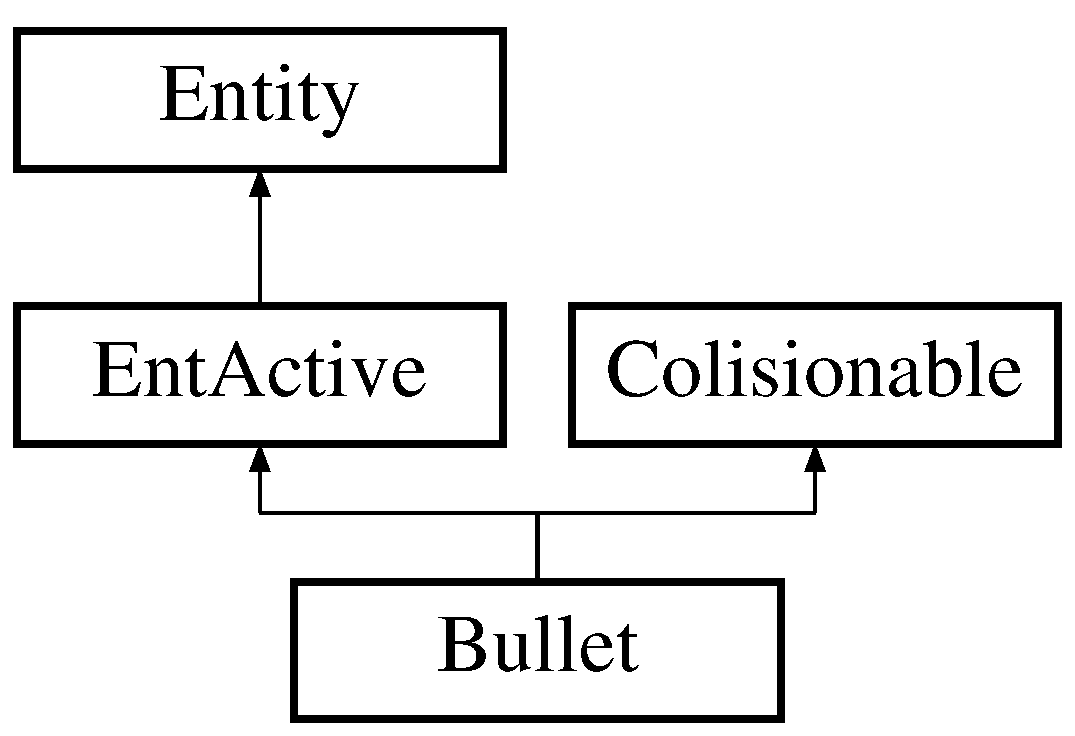
\includegraphics[height=3.000000cm]{classBullet}
\end{center}
\end{figure}
\subsection*{Métodos públicos}
\begin{DoxyCompactItemize}
\item 
\hypertarget{classBullet_a28f66f8117c5db3ae465ef8722df9464}{{\bfseries Bullet} (const sf\-::\-Texture \&tex, bool cen)}\label{classBullet_a28f66f8117c5db3ae465ef8722df9464}

\item 
\hypertarget{classBullet_a66d17e68781cf0b136b4866f7591dc5a}{{\bfseries Bullet} (const sf\-::\-Texture \&tex, const \hyperlink{classVector}{Vector} \&pos, const \hyperlink{classVector}{Vector} \&vel=\hyperlink{classVector}{Vector}(0.f, 0.f), const \hyperlink{classVector}{Vector} \&maxvel=\hyperlink{classVector}{Vector}(600.f, 600.f), bool cen=true)}\label{classBullet_a66d17e68781cf0b136b4866f7591dc5a}

\item 
\hypertarget{classBullet_a22e572e4d102f86b68db3bfed3532b6d}{{\bfseries Bullet} (const \hyperlink{classBullet}{Bullet} \&orig)}\label{classBullet_a22e572e4d102f86b68db3bfed3532b6d}

\item 
virtual void \hyperlink{classBullet_af27d3a1699386dcd15bcb4a338b8b993}{Draw} (\hyperlink{classRenderWindow}{Render\-Window} \&window, float inter)
\begin{DoxyCompactList}\small\item\em Realiza un Draw Interpolado. \end{DoxyCompactList}\item 
\hypertarget{classBullet_a452c100efdd14343cb7e651477a4f7b5}{virtual void \hyperlink{classBullet_a452c100efdd14343cb7e651477a4f7b5}{Update} (const \hyperlink{classTime}{Time} \&elapsed\-Time)}\label{classBullet_a452c100efdd14343cb7e651477a4f7b5}

\begin{DoxyCompactList}\small\item\em Realizará un Update de la física, además el propio en las clases hijas. \end{DoxyCompactList}\item 
\hypertarget{classBullet_aff602c0a337b7a4290eb1dc0de729463}{void {\bfseries Add\-Time\-Elapsed} (const \hyperlink{classTime}{Time} \&time)}\label{classBullet_aff602c0a337b7a4290eb1dc0de729463}

\item 
\hypertarget{classBullet_ad68e706617b9e3f260329e767fd4cdb6}{\hyperlink{classTime}{Time} \& {\bfseries Get\-Time\-Elapsed} () const }\label{classBullet_ad68e706617b9e3f260329e767fd4cdb6}

\item 
\hypertarget{classBullet_aa1e5f892a1a175f04bc67e2fc993a619}{virtual void {\bfseries On\-Colision} (Colision\-::\-Type type, const \hyperlink{classRectangle}{Rectangle} \&rec)}\label{classBullet_aa1e5f892a1a175f04bc67e2fc993a619}

\end{DoxyCompactItemize}
\subsection*{Atributos públicos}
\begin{DoxyCompactItemize}
\item 
\hypertarget{classBullet_a5a392a85e958fe7dabebd1950bcf07aa}{bool {\bfseries affect\-Gravity} =false}\label{classBullet_a5a392a85e958fe7dabebd1950bcf07aa}

\item 
\hypertarget{classBullet_a1cad8c80e63d13da57b563b8e8e3f79e}{float {\bfseries damage} = 20.f}\label{classBullet_a1cad8c80e63d13da57b563b8e8e3f79e}

\end{DoxyCompactItemize}
\subsection*{Otros miembros heredados}


\subsection{Documentación de las funciones miembro}
\hypertarget{classBullet_af27d3a1699386dcd15bcb4a338b8b993}{\index{Bullet@{Bullet}!Draw@{Draw}}
\index{Draw@{Draw}!Bullet@{Bullet}}
\subsubsection[{Draw}]{\setlength{\rightskip}{0pt plus 5cm}void Bullet\-::\-Draw (
\begin{DoxyParamCaption}
\item[{{\bf Render\-Window} \&}]{window, }
\item[{float}]{inter}
\end{DoxyParamCaption}
)\hspace{0.3cm}{\ttfamily [virtual]}}}\label{classBullet_af27d3a1699386dcd15bcb4a338b8b993}


Realiza un Draw Interpolado. 

Dibujado con interpolacion. 

Reimplementado de \hyperlink{classEntActive_a658baff215085c022d8a019269185a66}{Ent\-Active}.



La documentación para esta clase fue generada a partir de los siguientes ficheros\-:\begin{DoxyCompactItemize}
\item 
/home/linuxero/\-Net\-Beans\-Projects/prueba\-\_\-colisiones/\-Clases/Bullet.\-h\item 
/home/linuxero/\-Net\-Beans\-Projects/prueba\-\_\-colisiones/\-Clases/Bullet.\-cpp\end{DoxyCompactItemize}

\hypertarget{classClock}{\section{Referencia de la Clase Clock}
\label{classClock}\index{Clock@{Clock}}
}
\subsection*{Métodos públicos}
\begin{DoxyCompactItemize}
\item 
\hypertarget{classClock_a5a33622744878d233352e2ddde5acf98}{{\bfseries Clock} (const \hyperlink{classClock}{Clock} \&orig)}\label{classClock_a5a33622744878d233352e2ddde5acf98}

\item 
\hypertarget{classClock_a5909f7677c453f589ef109c5e30251ab}{\hyperlink{classTime}{Time} {\bfseries Restart} ()}\label{classClock_a5909f7677c453f589ef109c5e30251ab}

\item 
\hypertarget{classClock_aca8f3ca2f9b36eb348217747b4413484}{\hyperlink{classTime}{Time} {\bfseries Get\-Elapsed\-Time} () const }\label{classClock_aca8f3ca2f9b36eb348217747b4413484}

\end{DoxyCompactItemize}
\subsection*{Atributos públicos}
\begin{DoxyCompactItemize}
\item 
\hypertarget{classClock_adff8b3a1419c696ec7e98fd2499ea6ef}{sf\-::\-Clock $\ast$ {\bfseries clock}}\label{classClock_adff8b3a1419c696ec7e98fd2499ea6ef}

\end{DoxyCompactItemize}


La documentación para esta clase fue generada a partir de los siguientes ficheros\-:\begin{DoxyCompactItemize}
\item 
/home/linuxero/\-Net\-Beans\-Projects/prueba\-\_\-colisiones/\-Clases/Clock.\-h\item 
/home/linuxero/\-Net\-Beans\-Projects/prueba\-\_\-colisiones/\-Clases/Clock.\-cpp\end{DoxyCompactItemize}

\hypertarget{classColisionable}{\section{Referencia de la Clase Colisionable}
\label{classColisionable}\index{Colisionable@{Colisionable}}
}
Diagrama de herencias de Colisionable\begin{figure}[H]
\begin{center}
\leavevmode
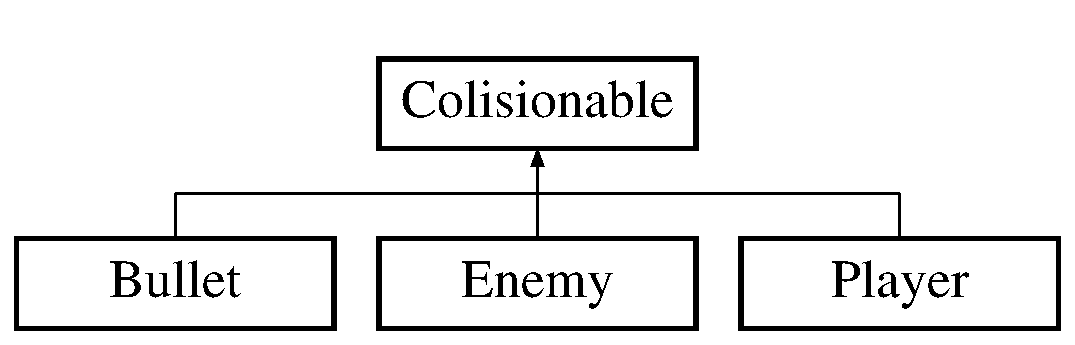
\includegraphics[height=2.000000cm]{classColisionable}
\end{center}
\end{figure}
\subsection*{Métodos públicos}
\begin{DoxyCompactItemize}
\item 
\hypertarget{classColisionable_a851878fb3a93420ca0cbec4605dbe2e1}{{\bfseries Colisionable} (\hyperlink{classEntity}{Entity} $\ast$ent)}\label{classColisionable_a851878fb3a93420ca0cbec4605dbe2e1}

\item 
\hypertarget{classColisionable_ac170a1b17950bb9f72b01261e474d65f}{{\bfseries Colisionable} (const \hyperlink{classColisionable}{Colisionable} \&orig)}\label{classColisionable_ac170a1b17950bb9f72b01261e474d65f}

\item 
\hypertarget{classColisionable_aecb15e3d0280c07f16fb12ee7c399b43}{virtual const std\-::string {\bfseries Get\-Class\-Name} ()}\label{classColisionable_aecb15e3d0280c07f16fb12ee7c399b43}

\item 
\hypertarget{classColisionable_a49c839ada10fd0b51ae3b04da9fc5831}{\hyperlink{classRectangle}{Rectangle} {\bfseries Get\-Previous\-Rect} (const \hyperlink{classTime}{Time} \&elapsed\-Time, \hyperlink{classEntActive}{Ent\-Active} $\ast$ent) const }\label{classColisionable_a49c839ada10fd0b51ae3b04da9fc5831}

\item 
\hypertarget{classColisionable_a8753bbdd0249f54cdd2b20177d40e55e}{int \hyperlink{classColisionable_a8753bbdd0249f54cdd2b20177d40e55e}{Create\-Rectangle} (float x, float y, float width, float height)}\label{classColisionable_a8753bbdd0249f54cdd2b20177d40e55e}

\begin{DoxyCompactList}\small\item\em Creará un Rectángulo con los valores R\-E\-L\-A\-T\-I\-V\-O\-S de los parámetros (entre 0.\-f y 1.\-f) \end{DoxyCompactList}\item 
\hypertarget{classColisionable_a2fd73529e7ac9eb9977c32dbed5825e9}{\hyperlink{classRectangle}{Rectangle} {\bfseries Get\-Absolute\-Rectangle} (const \hyperlink{classEntity}{Entity} \&ent, const \hyperlink{classRectangle}{Rectangle} \&rec\-Relative)}\label{classColisionable_a2fd73529e7ac9eb9977c32dbed5825e9}

\item 
\hypertarget{classColisionable_a7341c612181dcaedaa140f47bc4ddea4}{std\-::vector$<$ \hyperlink{classRectangle}{Rectangle} $>$ {\bfseries Get\-Absolute\-Rectangles} (const \hyperlink{classEntity}{Entity} \&ent)}\label{classColisionable_a7341c612181dcaedaa140f47bc4ddea4}

\item 
\hypertarget{classColisionable_ab4d827408fd136a4ccd1d188492d907e}{virtual bool {\bfseries Check\-Colision} (const \hyperlink{classColisionable}{Colisionable} \&ent)}\label{classColisionable_ab4d827408fd136a4ccd1d188492d907e}

\item 
\hypertarget{classColisionable_a568ec4a1fb2d412c19a1416309b967b5}{virtual bool {\bfseries Check\-Colision} (const \hyperlink{classRectangle}{Rectangle} \&rec)}\label{classColisionable_a568ec4a1fb2d412c19a1416309b967b5}

\item 
\hypertarget{classColisionable_a6d799e9995e2e635461e66d74bf8fd5c}{virtual std\-::vector$<$ \hyperlink{classVector}{Vector} $>$ {\bfseries Check\-Deep\-Colision} (const \hyperlink{classColisionable}{Colisionable} \&ent)}\label{classColisionable_a6d799e9995e2e635461e66d74bf8fd5c}

\item 
\hypertarget{classColisionable_ac2a8556867c95d6174965768dc7b7c2f}{virtual std\-::vector$<$ int $>$ {\bfseries Check\-Deep\-Colision} (const \hyperlink{classRectangle}{Rectangle} \&rec)}\label{classColisionable_ac2a8556867c95d6174965768dc7b7c2f}

\item 
\hypertarget{classColisionable_a1058ee9817cbce361a5af71a9b29d40a}{virtual Colision\-::\-Type {\bfseries Type\-Of\-Colision} (const \hyperlink{classColisionable}{Colisionable} \&ent, int index\-From, int index\-To, const \hyperlink{classTime}{Time} \&elapsed\-Time)}\label{classColisionable_a1058ee9817cbce361a5af71a9b29d40a}

\item 
\hypertarget{classColisionable_abf660cb4fb76c044424efbd06f7c1e97}{virtual Colision\-::\-Type {\bfseries Type\-Of\-Colision} (const \hyperlink{classRectangle}{Rectangle} \&rec, int index, const \hyperlink{classTime}{Time} \&elapsed\-Time)}\label{classColisionable_abf660cb4fb76c044424efbd06f7c1e97}

\item 
\hypertarget{classColisionable_a7863f7dfc211812f380547bcd73b7a41}{virtual Colision\-::\-Type {\bfseries Type\-Of\-Colision} (const \hyperlink{classColisionable}{Colisionable} \&ent, const \hyperlink{classTime}{Time} \&elapsed\-Time)}\label{classColisionable_a7863f7dfc211812f380547bcd73b7a41}

\item 
\hypertarget{classColisionable_abce19bbf1e92890ffc54abbc892adbc1}{virtual Colision\-::\-Type {\bfseries Type\-Of\-Colision} (const \hyperlink{classRectangle}{Rectangle} \&rec, const \hyperlink{classTime}{Time} \&elapsed\-Time)}\label{classColisionable_abce19bbf1e92890ffc54abbc892adbc1}

\item 
\hypertarget{classColisionable_a5aa4d9e35ede30c4cd1d68a0b946d72c}{virtual void {\bfseries On\-Colision} (Colision\-::\-Type type, const \hyperlink{classRectangle}{Rectangle} \&rec)=0}\label{classColisionable_a5aa4d9e35ede30c4cd1d68a0b946d72c}

\item 
\hypertarget{classColisionable_a5826db7bec1ff455bf5570097b3c96cd}{virtual void {\bfseries Reset\-Can} ()}\label{classColisionable_a5826db7bec1ff455bf5570097b3c96cd}

\item 
\hypertarget{classColisionable_a9dbbdaf66b24a1203e2e67fc8c6bd9e5}{virtual void {\bfseries Substract\-Distance} (Colision\-::\-Type type, \hyperlink{classEntActive}{Ent\-Active} $\ast$ent, const \hyperlink{classRectangle}{Rectangle} \&rec)}\label{classColisionable_a9dbbdaf66b24a1203e2e67fc8c6bd9e5}

\end{DoxyCompactItemize}
\subsection*{Atributos públicos}
\begin{DoxyCompactItemize}
\item 
\hypertarget{classColisionable_a07729cf3ff6ed199132dd336a87887a7}{float {\bfseries force\-Jump} = 500.f}\label{classColisionable_a07729cf3ff6ed199132dd336a87887a7}

\item 
\hypertarget{classColisionable_a7742961d8b1f1a22d930bd44da27b064}{bool {\bfseries can\-Left}}\label{classColisionable_a7742961d8b1f1a22d930bd44da27b064}

\item 
\hypertarget{classColisionable_ac2faafc0b6d7e8d30e1022ebc87c206f}{bool {\bfseries can\-Right}}\label{classColisionable_ac2faafc0b6d7e8d30e1022ebc87c206f}

\item 
\hypertarget{classColisionable_ad311d7e49f065e66d479be76722770ae}{bool {\bfseries can\-Jump}}\label{classColisionable_ad311d7e49f065e66d479be76722770ae}

\end{DoxyCompactItemize}


La documentación para esta clase fue generada a partir de los siguientes ficheros\-:\begin{DoxyCompactItemize}
\item 
/home/linuxero/\-Net\-Beans\-Projects/prueba\-\_\-colisiones/\-Clases/Colisionable.\-h\item 
/home/linuxero/\-Net\-Beans\-Projects/prueba\-\_\-colisiones/\-Clases/Colisionable.\-cpp\end{DoxyCompactItemize}

\hypertarget{classEnemy}{\section{Referencia de la Clase Enemy}
\label{classEnemy}\index{Enemy@{Enemy}}
}
Diagrama de herencias de Enemy\begin{figure}[H]
\begin{center}
\leavevmode
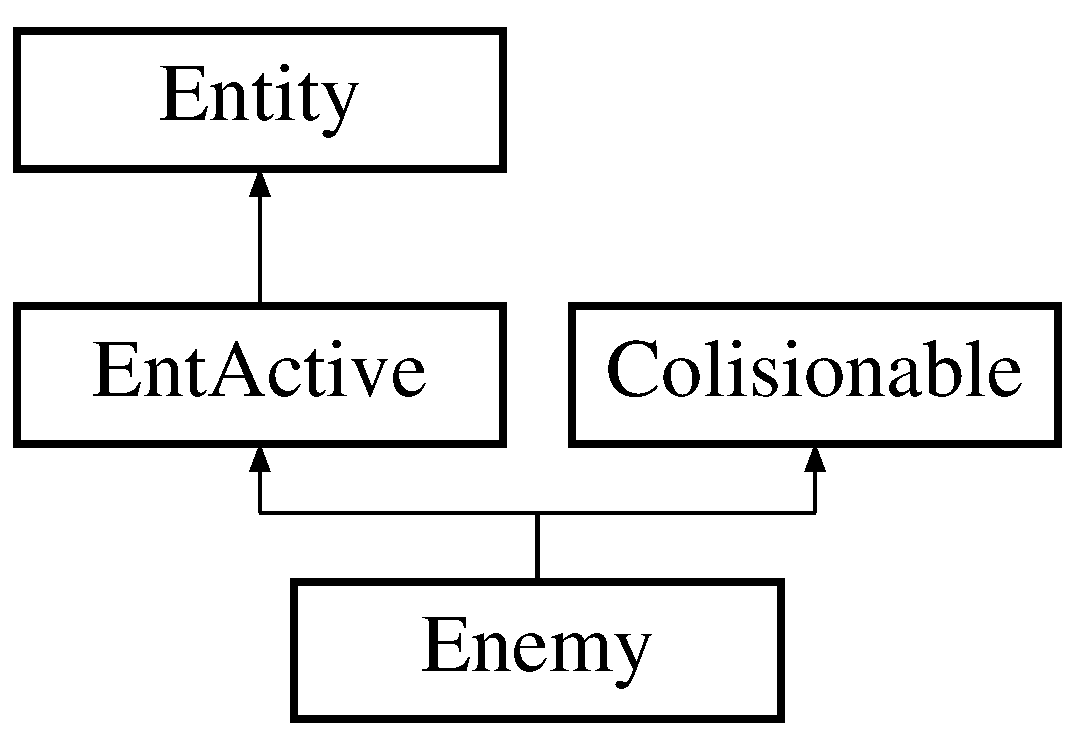
\includegraphics[height=3.000000cm]{classEnemy}
\end{center}
\end{figure}
\subsection*{Métodos públicos}
\begin{DoxyCompactItemize}
\item 
\hypertarget{classEnemy_a61d6ab34a7c18bde3480468e98cf9ba4}{{\bfseries Enemy} (const sf\-::\-Texture \&tex, bool cen=true)}\label{classEnemy_a61d6ab34a7c18bde3480468e98cf9ba4}

\item 
\hypertarget{classEnemy_a59302df40922f5b0193c16b5650fb3c9}{{\bfseries Enemy} (const sf\-::\-Texture \&tex, const \hyperlink{classVector}{Vector} \&pos, const \hyperlink{classVector}{Vector} \&vel=\hyperlink{classVector}{Vector}(0.f, 0.f), const \hyperlink{classVector}{Vector} \&maxvel=\hyperlink{classVector}{Vector}(600.f, 600.f), bool cen=true)}\label{classEnemy_a59302df40922f5b0193c16b5650fb3c9}

\item 
\hypertarget{classEnemy_a9719f9eedddb5950fc1e522051a93d93}{{\bfseries Enemy} (const \hyperlink{classEnemy}{Enemy} \&orig)}\label{classEnemy_a9719f9eedddb5950fc1e522051a93d93}

\item 
\hypertarget{classEnemy_a6f34d90e9ef3b2e94b2093c0d7113f13}{virtual const std\-::string {\bfseries Get\-Class\-Name} ()}\label{classEnemy_a6f34d90e9ef3b2e94b2093c0d7113f13}

\item 
virtual void \hyperlink{classEnemy_a9a34d38fac00edea2f45a9084bdfe1f6}{Draw} (\hyperlink{classRenderWindow}{Render\-Window} \&window, float inter)
\begin{DoxyCompactList}\small\item\em Realiza un Draw Interpolado. \end{DoxyCompactList}\item 
\hypertarget{classEnemy_a7c26659cca9c7efdae3ffad6af20df5f}{virtual void \hyperlink{classEnemy_a7c26659cca9c7efdae3ffad6af20df5f}{Update} (const \hyperlink{classTime}{Time} \&elapsed\-Time)}\label{classEnemy_a7c26659cca9c7efdae3ffad6af20df5f}

\begin{DoxyCompactList}\small\item\em Realizará un Update de la física, además el propio en las clases hijas. \end{DoxyCompactList}\item 
\hypertarget{classEnemy_a754ebd8eb9db54ec38695a72dd6d801b}{void {\bfseries On\-Colision} (Colision\-::\-Type type, const \hyperlink{classRectangle}{Rectangle} \&rec)}\label{classEnemy_a754ebd8eb9db54ec38695a72dd6d801b}

\end{DoxyCompactItemize}
\subsection*{Atributos públicos}
\begin{DoxyCompactItemize}
\item 
\hypertarget{classEnemy_aee0e2aa489b58e73c849034893fa0d33}{float {\bfseries life} =100.f}\label{classEnemy_aee0e2aa489b58e73c849034893fa0d33}

\end{DoxyCompactItemize}
\subsection*{Otros miembros heredados}


\subsection{Documentación de las funciones miembro}
\hypertarget{classEnemy_a9a34d38fac00edea2f45a9084bdfe1f6}{\index{Enemy@{Enemy}!Draw@{Draw}}
\index{Draw@{Draw}!Enemy@{Enemy}}
\subsubsection[{Draw}]{\setlength{\rightskip}{0pt plus 5cm}void Enemy\-::\-Draw (
\begin{DoxyParamCaption}
\item[{{\bf Render\-Window} \&}]{window, }
\item[{float}]{inter}
\end{DoxyParamCaption}
)\hspace{0.3cm}{\ttfamily [virtual]}}}\label{classEnemy_a9a34d38fac00edea2f45a9084bdfe1f6}


Realiza un Draw Interpolado. 

Dibujado con interpolacion. 

Reimplementado de \hyperlink{classEntActive_a658baff215085c022d8a019269185a66}{Ent\-Active}.



La documentación para esta clase fue generada a partir de los siguientes ficheros\-:\begin{DoxyCompactItemize}
\item 
/home/linuxero/\-Net\-Beans\-Projects/prueba\-\_\-colisiones/\-Clases/Enemy.\-h\item 
/home/linuxero/\-Net\-Beans\-Projects/prueba\-\_\-colisiones/\-Clases/Enemy.\-cpp\end{DoxyCompactItemize}

\hypertarget{classEntActive}{\section{Referencia de la Clase Ent\-Active}
\label{classEntActive}\index{Ent\-Active@{Ent\-Active}}
}
Diagrama de herencias de Ent\-Active\begin{figure}[H]
\begin{center}
\leavevmode
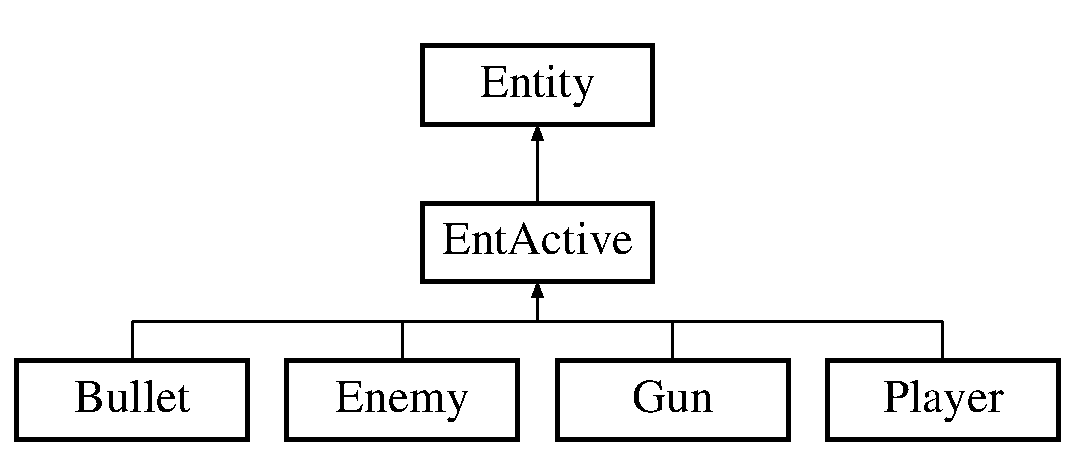
\includegraphics[height=3.000000cm]{classEntActive}
\end{center}
\end{figure}
\subsection*{Métodos públicos}
\begin{DoxyCompactItemize}
\item 
\hypertarget{classEntActive_a81931d25b400fc5e130105485faa709f}{{\bfseries Ent\-Active} (const sf\-::\-Texture \&tex, bool cen=true)}\label{classEntActive_a81931d25b400fc5e130105485faa709f}

\item 
\hypertarget{classEntActive_a5d2b8ee5788d63b5ee728d260baa142d}{{\bfseries Ent\-Active} (const sf\-::\-Texture \&tex, const \hyperlink{classVector}{Vector} \&pos, const \hyperlink{classVector}{Vector} \&vel=\hyperlink{classVector}{Vector}(0.f, 0.f), const \hyperlink{classVector}{Vector} \&maxvel=\hyperlink{classVector}{Vector}(600.f, 600.f), bool cen=true)}\label{classEntActive_a5d2b8ee5788d63b5ee728d260baa142d}

\item 
\hypertarget{classEntActive_a80e6db9b0c09d4e7341bf594644537d6}{{\bfseries Ent\-Active} (const \hyperlink{classEntActive}{Ent\-Active} \&orig)}\label{classEntActive_a80e6db9b0c09d4e7341bf594644537d6}

\item 
virtual void \hyperlink{classEntActive_a658baff215085c022d8a019269185a66}{Draw} (\hyperlink{classRenderWindow}{Render\-Window} \&window, float inter)
\begin{DoxyCompactList}\small\item\em Realiza un Draw Interpolado. \end{DoxyCompactList}\item 
\hypertarget{classEntActive_a5bd08db0c510184d069cd48ee037cbb5}{virtual void \hyperlink{classEntActive_a5bd08db0c510184d069cd48ee037cbb5}{Update} (const \hyperlink{classTime}{Time} \&elapsed\-Time)}\label{classEntActive_a5bd08db0c510184d069cd48ee037cbb5}

\begin{DoxyCompactList}\small\item\em Realizará un Update de la física, además el propio en las clases hijas. \end{DoxyCompactList}\item 
\hypertarget{classEntActive_a7c0d9232f28e3c8f697666a13eedf1fd}{\hyperlink{classVector}{Vector} \& {\bfseries Get\-Position} () const }\label{classEntActive_a7c0d9232f28e3c8f697666a13eedf1fd}

\item 
\hypertarget{classEntActive_a2b8fc413a6cf15005c3d5df61df9bf68}{\hyperlink{classVector}{Vector} \& {\bfseries Get\-Previous\-Position} () const }\label{classEntActive_a2b8fc413a6cf15005c3d5df61df9bf68}

\item 
\hypertarget{classEntActive_a81d1d29c10269c1e5e13b08d5c8b3500}{\hyperlink{classVector}{Vector} \& {\bfseries Get\-Speed} () const }\label{classEntActive_a81d1d29c10269c1e5e13b08d5c8b3500}

\item 
\hypertarget{classEntActive_a1e04391aa346f92d82dfc8f4b28ebf42}{\hyperlink{classVector}{Vector} \& {\bfseries Get\-Max\-Speed} () const }\label{classEntActive_a1e04391aa346f92d82dfc8f4b28ebf42}

\item 
\hypertarget{classEntActive_a220de2b9c4114cf618a0a2686c491534}{\hyperlink{classVector}{Vector} \& {\bfseries Get\-Gravity} () const }\label{classEntActive_a220de2b9c4114cf618a0a2686c491534}

\item 
\hypertarget{classEntActive_adea1929ea05822a5b7a158a2f32d6081}{void {\bfseries Set\-Position} (float x, float y)}\label{classEntActive_adea1929ea05822a5b7a158a2f32d6081}

\item 
\hypertarget{classEntActive_a961dd9abd27dbfd3e3d995bc496db838}{void {\bfseries Set\-Position} (const \hyperlink{classVector}{Vector} \&v)}\label{classEntActive_a961dd9abd27dbfd3e3d995bc496db838}

\item 
\hypertarget{classEntActive_ade0700e3aeb97d97575f8e9e8d266284}{void {\bfseries Set\-Speed} (float x, float y)}\label{classEntActive_ade0700e3aeb97d97575f8e9e8d266284}

\item 
\hypertarget{classEntActive_a43c881770b61f5fe51a062017dcd8d77}{void {\bfseries Set\-Speed} (const \hyperlink{classVector}{Vector} \&v)}\label{classEntActive_a43c881770b61f5fe51a062017dcd8d77}

\item 
\hypertarget{classEntActive_a637290b5f2c564af4143f6ac6f650759}{void {\bfseries Set\-Max\-Speed} (float x, float y)}\label{classEntActive_a637290b5f2c564af4143f6ac6f650759}

\item 
\hypertarget{classEntActive_ab56a2a10c81ee660d2374bbd0cf4e6c7}{void {\bfseries Set\-Max\-Speed} (const \hyperlink{classVector}{Vector} \&v)}\label{classEntActive_ab56a2a10c81ee660d2374bbd0cf4e6c7}

\item 
\hypertarget{classEntActive_a0a5e9087aae52af8fd4203ce9fe5f035}{void {\bfseries Set\-Gravity} (const \hyperlink{classVector}{Vector} \&g)}\label{classEntActive_a0a5e9087aae52af8fd4203ce9fe5f035}

\end{DoxyCompactItemize}
\subsection*{Atributos públicos}
\begin{DoxyCompactItemize}
\item 
\hypertarget{classEntActive_aa79d76a4cef52b2a40c76597e8d3d304}{float {\bfseries factor\-Speed} = 400.f}\label{classEntActive_aa79d76a4cef52b2a40c76597e8d3d304}

\item 
\hypertarget{classEntActive_a3f9970329246bf5e468df19f8fa4bd81}{float {\bfseries factor\-Gravity} = 800.f}\label{classEntActive_a3f9970329246bf5e468df19f8fa4bd81}

\item 
\hypertarget{classEntActive_aacfe6ed7ec684a8d75440043be0cf4cb}{bool {\bfseries affect\-Gravity} = true}\label{classEntActive_aacfe6ed7ec684a8d75440043be0cf4cb}

\end{DoxyCompactItemize}
\subsection*{Atributos protegidos}
\begin{DoxyCompactItemize}
\item 
\hypertarget{classEntActive_a6942ffeccdffebb8a286b13815699d11}{\hyperlink{classPhysicsState}{Physics\-State} $\ast$ {\bfseries physics\-State}}\label{classEntActive_a6942ffeccdffebb8a286b13815699d11}

\item 
\hypertarget{classEntActive_adb6491b21f10ec565c645de1a0abb33a}{\hyperlink{classRenderState}{Render\-State} $\ast$ {\bfseries render\-State}}\label{classEntActive_adb6491b21f10ec565c645de1a0abb33a}

\end{DoxyCompactItemize}


\subsection{Documentación de las funciones miembro}
\hypertarget{classEntActive_a658baff215085c022d8a019269185a66}{\index{Ent\-Active@{Ent\-Active}!Draw@{Draw}}
\index{Draw@{Draw}!EntActive@{Ent\-Active}}
\subsubsection[{Draw}]{\setlength{\rightskip}{0pt plus 5cm}void Ent\-Active\-::\-Draw (
\begin{DoxyParamCaption}
\item[{{\bf Render\-Window} \&}]{window, }
\item[{float}]{inter}
\end{DoxyParamCaption}
)\hspace{0.3cm}{\ttfamily [virtual]}}}\label{classEntActive_a658baff215085c022d8a019269185a66}


Realiza un Draw Interpolado. 

Dibujado con interpolacion. 

Reimplementado en \hyperlink{classPlayer_a6fa2109456d203d45b0460fa53ff247b}{Player}, \hyperlink{classEnemy_a9a34d38fac00edea2f45a9084bdfe1f6}{Enemy}, \hyperlink{classGun_a70271085b85f4cfa2cf8e74975e7fef9}{Gun} y \hyperlink{classBullet_af27d3a1699386dcd15bcb4a338b8b993}{Bullet}.



La documentación para esta clase fue generada a partir de los siguientes ficheros\-:\begin{DoxyCompactItemize}
\item 
/home/linuxero/\-Net\-Beans\-Projects/prueba\-\_\-colisiones/\-Clases/Ent\-Active.\-h\item 
/home/linuxero/\-Net\-Beans\-Projects/prueba\-\_\-colisiones/\-Clases/Ent\-Active.\-cpp\end{DoxyCompactItemize}

\hypertarget{classEntity}{\section{Referencia de la Clase Entity}
\label{classEntity}\index{Entity@{Entity}}
}
Diagrama de herencias de Entity\begin{figure}[H]
\begin{center}
\leavevmode
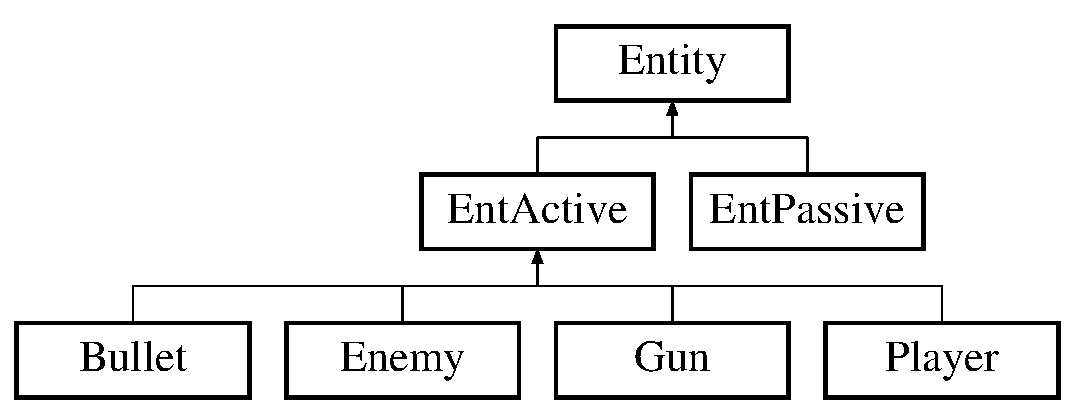
\includegraphics[height=3.000000cm]{classEntity}
\end{center}
\end{figure}
\subsection*{Métodos públicos}
\begin{DoxyCompactItemize}
\item 
\hypertarget{classEntity_a003b768b26fc58c86db1bebf4d9e6dc0}{{\bfseries Entity} (const sf\-::\-Texture \&tex, bool cen=true)}\label{classEntity_a003b768b26fc58c86db1bebf4d9e6dc0}

\item 
\hypertarget{classEntity_a9de139ff12775dd95fb80bec08247de7}{{\bfseries Entity} (const \hyperlink{classEntity}{Entity} \&orig)}\label{classEntity_a9de139ff12775dd95fb80bec08247de7}

\item 
\hypertarget{classEntity_a4c91428df1de64d453403259528d0cf5}{virtual const std\-::string {\bfseries Get\-Class\-Name} ()}\label{classEntity_a4c91428df1de64d453403259528d0cf5}

\item 
\hypertarget{classEntity_a8bee0e0ef049bede8b99ed8adf449e05}{virtual void {\bfseries Update} (const \hyperlink{classTime}{Time} \&elapsed\-Time)=0}\label{classEntity_a8bee0e0ef049bede8b99ed8adf449e05}

\item 
\hypertarget{classEntity_aae98125c6edca41264a3992987937865}{\hyperlink{classSprite}{Sprite} $\ast$ {\bfseries Get\-Sprite} () const }\label{classEntity_aae98125c6edca41264a3992987937865}

\item 
\hypertarget{classEntity_a0910fd995e8c73bf6c48d42c04e15ec3}{virtual void {\bfseries Set\-Position} (const \hyperlink{classVector}{Vector} \&v)=0}\label{classEntity_a0910fd995e8c73bf6c48d42c04e15ec3}

\item 
\hypertarget{classEntity_a1a88f8b1352ab1e53faffcfab9931a61}{virtual \hyperlink{classVector}{Vector} \& {\bfseries Get\-Position} () const =0}\label{classEntity_a1a88f8b1352ab1e53faffcfab9931a61}

\end{DoxyCompactItemize}
\subsection*{Atributos protegidos}
\begin{DoxyCompactItemize}
\item 
\hypertarget{classEntity_a4da30cea569f19c66c033358e1e99c04}{\hyperlink{classSprite}{Sprite} $\ast$ {\bfseries sprite}}\label{classEntity_a4da30cea569f19c66c033358e1e99c04}

\end{DoxyCompactItemize}


La documentación para esta clase fue generada a partir de los siguientes ficheros\-:\begin{DoxyCompactItemize}
\item 
/home/linuxero/\-Net\-Beans\-Projects/prueba\-\_\-colisiones/\-Clases/Entity.\-h\item 
/home/linuxero/\-Net\-Beans\-Projects/prueba\-\_\-colisiones/\-Clases/Entity.\-cpp\end{DoxyCompactItemize}

\hypertarget{classEntPassive}{\section{Referencia de la Clase Ent\-Passive}
\label{classEntPassive}\index{Ent\-Passive@{Ent\-Passive}}
}
Diagrama de herencias de Ent\-Passive\begin{figure}[H]
\begin{center}
\leavevmode
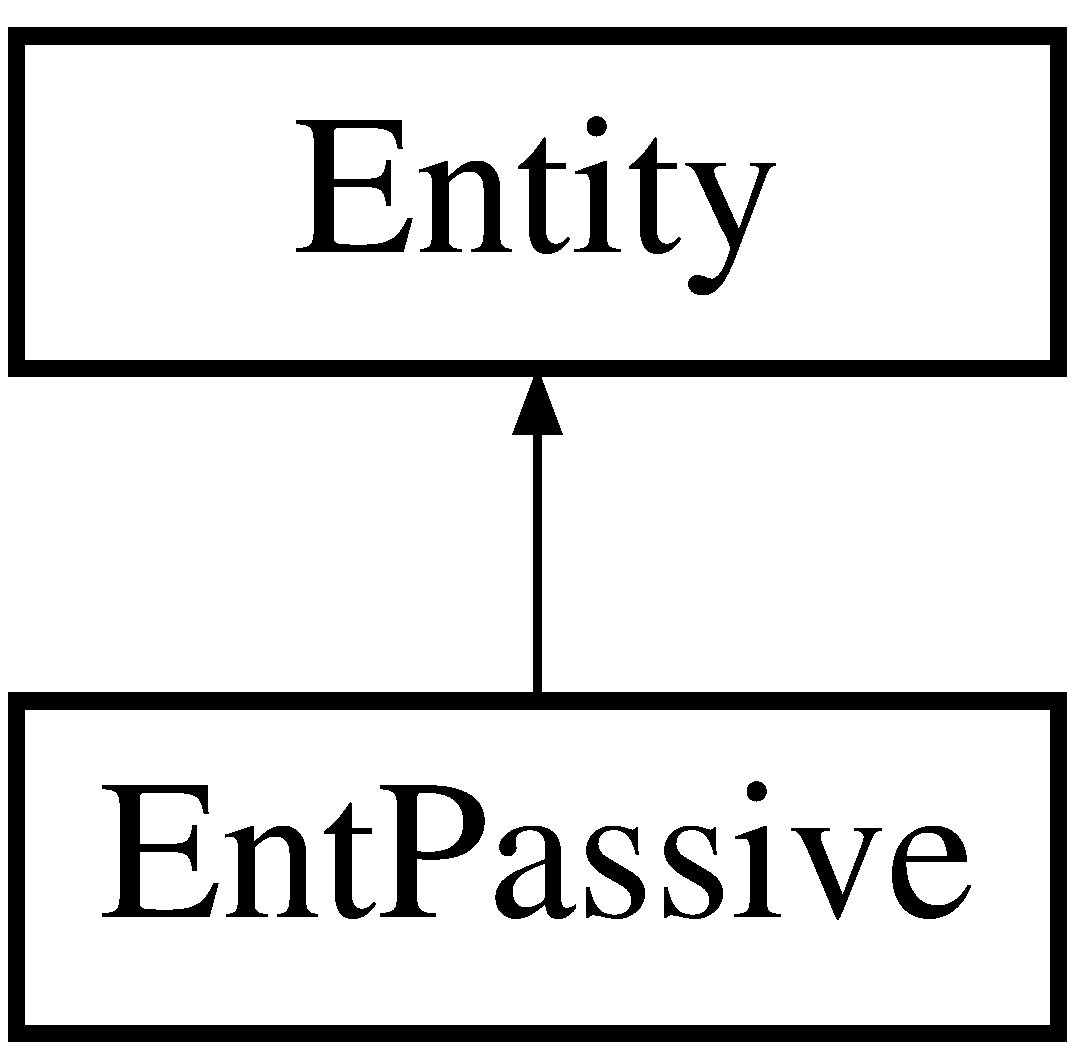
\includegraphics[height=2.000000cm]{classEntPassive}
\end{center}
\end{figure}
\subsection*{Métodos públicos}
\begin{DoxyCompactItemize}
\item 
\hypertarget{classEntPassive_a78cb6699f982f1eb3cf6b5192d38041e}{{\bfseries Ent\-Passive} (const sf\-::\-Texture \&tex, bool cen=true)}\label{classEntPassive_a78cb6699f982f1eb3cf6b5192d38041e}

\item 
\hypertarget{classEntPassive_a091c15b59be85d06872f1e6ac3d40f48}{{\bfseries Ent\-Passive} (const \hyperlink{classEntPassive}{Ent\-Passive} \&orig)}\label{classEntPassive_a091c15b59be85d06872f1e6ac3d40f48}

\item 
\hypertarget{classEntPassive_a116e6ea82a729055fce25902ca356d92}{virtual void \hyperlink{classEntPassive_a116e6ea82a729055fce25902ca356d92}{Draw} (\hyperlink{classRenderWindow}{Render\-Window} \&window)}\label{classEntPassive_a116e6ea82a729055fce25902ca356d92}

\begin{DoxyCompactList}\small\item\em Realiza un Draw simple. \end{DoxyCompactList}\item 
\hypertarget{classEntPassive_affdc25a39874ec0e9de12f650b9619ed}{virtual void \hyperlink{classEntPassive_affdc25a39874ec0e9de12f650b9619ed}{Update} (const \hyperlink{classTime}{Time} \&elapsed\-Time)}\label{classEntPassive_affdc25a39874ec0e9de12f650b9619ed}

\begin{DoxyCompactList}\small\item\em De momento no hará nada el update. \end{DoxyCompactList}\item 
\hypertarget{classEntPassive_aed5dc26f36af81a420a045b936b6485c}{void {\bfseries Set\-Position} (const \hyperlink{classVector}{Vector} \&v)}\label{classEntPassive_aed5dc26f36af81a420a045b936b6485c}

\item 
\hypertarget{classEntPassive_a76fafa1619fae14af0653de63bda7449}{\hyperlink{classVector}{Vector} {\bfseries Get\-Position} ()}\label{classEntPassive_a76fafa1619fae14af0653de63bda7449}

\item 
\hypertarget{classEntPassive_acceb3800d94b194628fc49dba5ca95df}{void {\bfseries Move} (\hyperlink{classVector}{Vector} v)}\label{classEntPassive_acceb3800d94b194628fc49dba5ca95df}

\end{DoxyCompactItemize}
\subsection*{Otros miembros heredados}


La documentación para esta clase fue generada a partir de los siguientes ficheros\-:\begin{DoxyCompactItemize}
\item 
/home/linuxero/\-Net\-Beans\-Projects/prueba\-\_\-colisiones/\-Clases/Ent\-Passive.\-h\item 
/home/linuxero/\-Net\-Beans\-Projects/prueba\-\_\-colisiones/\-Clases/Ent\-Passive.\-cpp\end{DoxyCompactItemize}

\hypertarget{classGun}{\section{Referencia de la Clase Gun}
\label{classGun}\index{Gun@{Gun}}
}
Diagrama de herencias de Gun\begin{figure}[H]
\begin{center}
\leavevmode
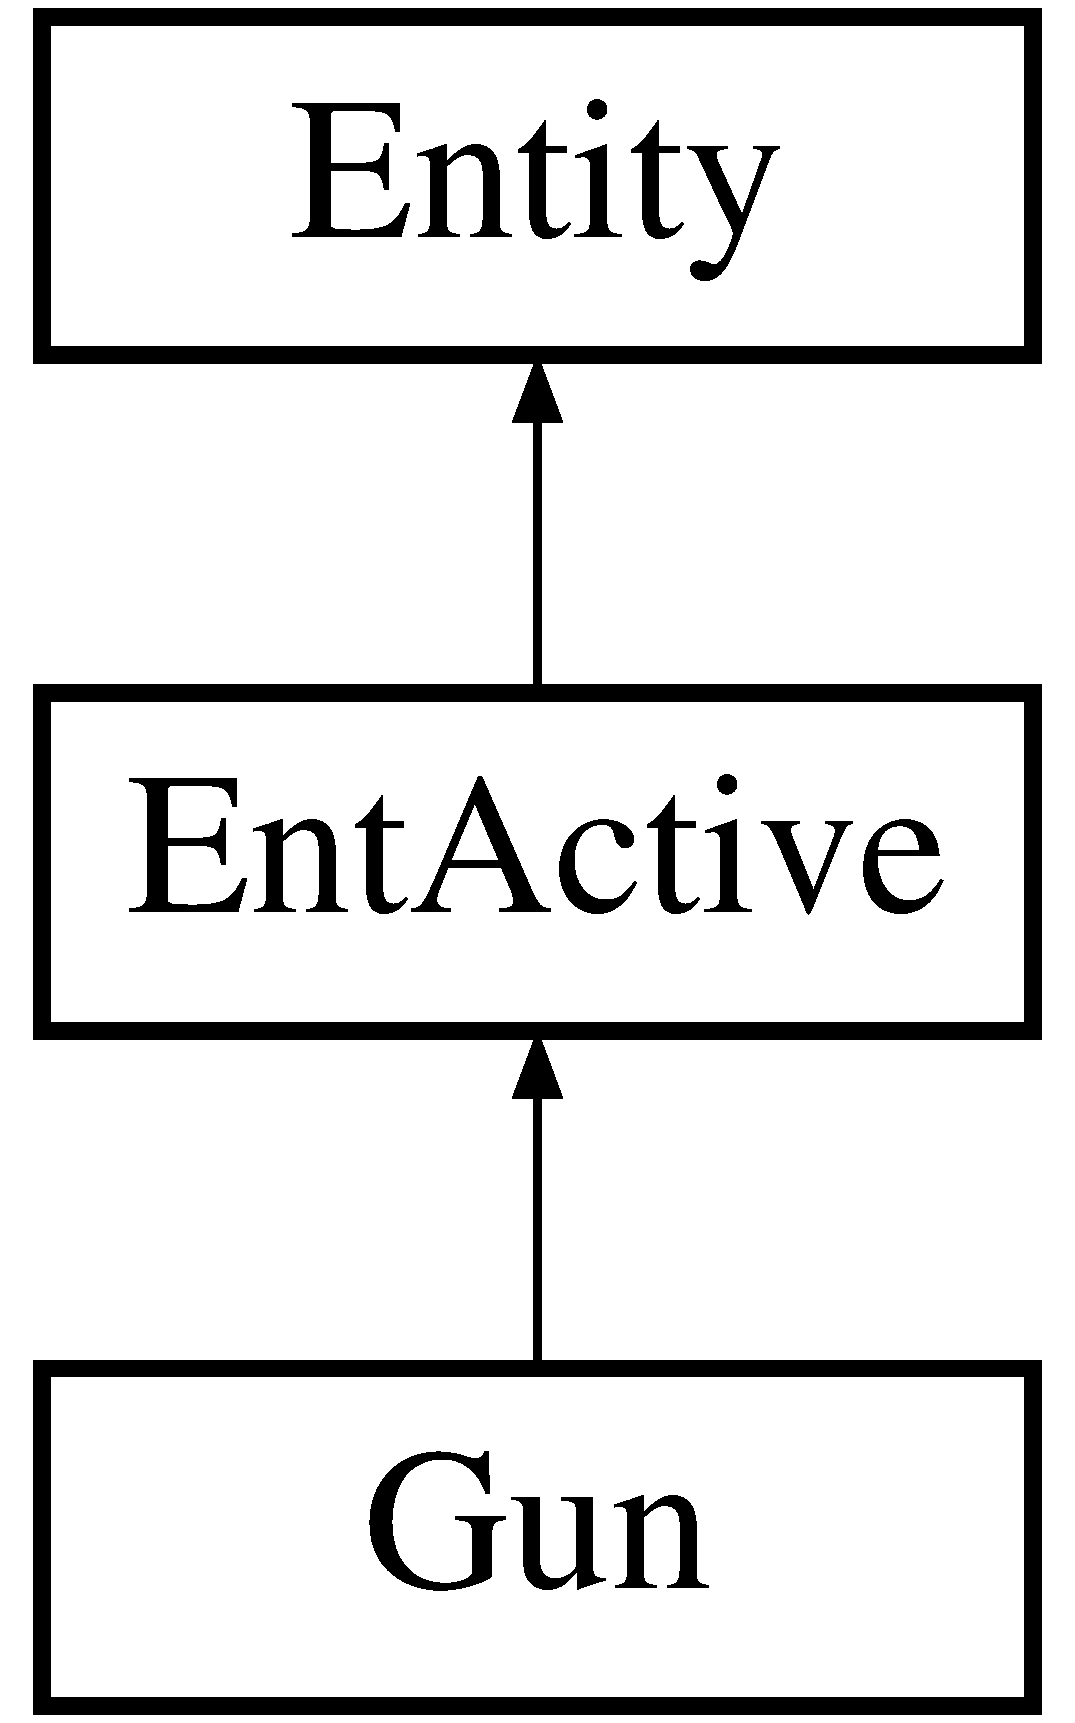
\includegraphics[height=3.000000cm]{classGun}
\end{center}
\end{figure}
\subsection*{Métodos públicos}
\begin{DoxyCompactItemize}
\item 
\hypertarget{classGun_add24df19b881b6944193889855490abf}{{\bfseries Gun} (const sf\-::\-Texture \&tex, bool cen=true)}\label{classGun_add24df19b881b6944193889855490abf}

\item 
\hypertarget{classGun_a17f769accaa9ad556047c628f00d9ad6}{{\bfseries Gun} (const sf\-::\-Texture \&tex, const \hyperlink{classVector}{Vector} \&pos, const \hyperlink{classVector}{Vector} \&vel=\hyperlink{classVector}{Vector}(0.f, 0.f), const \hyperlink{classVector}{Vector} \&maxvel=\hyperlink{classVector}{Vector}(600.f, 600.f), bool cen=true)}\label{classGun_a17f769accaa9ad556047c628f00d9ad6}

\item 
\hypertarget{classGun_a1e2c6e1776c3fe89592c012e020a6566}{{\bfseries Gun} (const \hyperlink{classGun}{Gun} \&orig)}\label{classGun_a1e2c6e1776c3fe89592c012e020a6566}

\item 
\hypertarget{classGun_a307c86c4feba903cd9672e17cb2d45f6}{virtual const std\-::string {\bfseries Get\-Class\-Name} ()}\label{classGun_a307c86c4feba903cd9672e17cb2d45f6}

\item 
virtual void \hyperlink{classGun_a70271085b85f4cfa2cf8e74975e7fef9}{Draw} (\hyperlink{classRenderWindow}{Render\-Window} \&window, float inter)
\begin{DoxyCompactList}\small\item\em Realiza un Draw Interpolado. \end{DoxyCompactList}\item 
\hypertarget{classGun_a888633a4af0a2d136ef2c366794d1544}{virtual void \hyperlink{classGun_a888633a4af0a2d136ef2c366794d1544}{Update} (const \hyperlink{classTime}{Time} \&elapsed\-Time)}\label{classGun_a888633a4af0a2d136ef2c366794d1544}

\begin{DoxyCompactList}\small\item\em Realizará un Update de la física, además el propio en las clases hijas. \end{DoxyCompactList}\item 
\hypertarget{classGun_af7bb838648ada8d4d730d3966264260f}{void {\bfseries Update} (\hyperlink{classEntActive}{Ent\-Active} $\ast$ent)}\label{classGun_af7bb838648ada8d4d730d3966264260f}

\item 
\hypertarget{classGun_a06d33bb4fc2d7937b05dd76caa7f3636}{virtual void {\bfseries Shot} (const \hyperlink{classVector}{Vector} \&speed, const \hyperlink{classVector}{Vector} \&pos)}\label{classGun_a06d33bb4fc2d7937b05dd76caa7f3636}

\item 
\hypertarget{classGun_a5d821a89ad458d1edd25fbf62d3f05fd}{void {\bfseries Set\-Times} (float life\-T, float reload\-T)}\label{classGun_a5d821a89ad458d1edd25fbf62d3f05fd}

\item 
\hypertarget{classGun_a4d7569f0a79398fd13cebf02ed859c06}{void {\bfseries Set\-Life\-Time} (float time)}\label{classGun_a4d7569f0a79398fd13cebf02ed859c06}

\item 
\hypertarget{classGun_ab3d0e69a52be0f11a38198d8a1d88536}{void {\bfseries Set\-Reload\-Time} (float time)}\label{classGun_ab3d0e69a52be0f11a38198d8a1d88536}

\item 
\hypertarget{classGun_a03bd2ed00d1fdb1767b78b0bec26ef05}{\hyperlink{classTime}{Time} \& {\bfseries Get\-Life\-Time} () const }\label{classGun_a03bd2ed00d1fdb1767b78b0bec26ef05}

\item 
\hypertarget{classGun_ad95a0db1e8df971a1eacefbff01f1b2c}{\hyperlink{classTime}{Time} \& {\bfseries Get\-Reload\-Time} () const }\label{classGun_ad95a0db1e8df971a1eacefbff01f1b2c}

\item 
\hypertarget{classGun_a033e18eb676db223a31a8c3a0371360e}{\hyperlink{classVector}{Vector} {\bfseries Get\-Relative\-Pos} () const }\label{classGun_a033e18eb676db223a31a8c3a0371360e}

\item 
\hypertarget{classGun_acd491acca640ffde2b1232ea381d1f77}{void {\bfseries Set\-Relative\-Pos} (float x, float y)}\label{classGun_acd491acca640ffde2b1232ea381d1f77}

\end{DoxyCompactItemize}
\subsection*{Otros miembros heredados}


\subsection{Documentación de las funciones miembro}
\hypertarget{classGun_a70271085b85f4cfa2cf8e74975e7fef9}{\index{Gun@{Gun}!Draw@{Draw}}
\index{Draw@{Draw}!Gun@{Gun}}
\subsubsection[{Draw}]{\setlength{\rightskip}{0pt plus 5cm}void Gun\-::\-Draw (
\begin{DoxyParamCaption}
\item[{{\bf Render\-Window} \&}]{window, }
\item[{float}]{inter}
\end{DoxyParamCaption}
)\hspace{0.3cm}{\ttfamily [virtual]}}}\label{classGun_a70271085b85f4cfa2cf8e74975e7fef9}


Realiza un Draw Interpolado. 

Dibujado con interpolacion. 

Reimplementado de \hyperlink{classEntActive_a658baff215085c022d8a019269185a66}{Ent\-Active}.



La documentación para esta clase fue generada a partir de los siguientes ficheros\-:\begin{DoxyCompactItemize}
\item 
/home/linuxero/\-Net\-Beans\-Projects/prueba\-\_\-colisiones/\-Clases/Gun.\-h\item 
/home/linuxero/\-Net\-Beans\-Projects/prueba\-\_\-colisiones/\-Clases/Gun.\-cpp\end{DoxyCompactItemize}

\hypertarget{classLevel}{\section{Referencia de la Clase Level}
\label{classLevel}\index{Level@{Level}}
}
\subsection*{Métodos públicos}
\begin{DoxyCompactItemize}
\item 
\hypertarget{classLevel_a620784c827607a855d4d6c8ac57755fa}{{\bfseries Level} (const \hyperlink{classLevel}{Level} \&orig)}\label{classLevel_a620784c827607a855d4d6c8ac57755fa}

\item 
\hypertarget{classLevel_a47703bc5d74e09ca0d9e19db6530c276}{void {\bfseries Add\-Colision} (\hyperlink{classRectangle}{Rectangle} $\ast$rec)}\label{classLevel_a47703bc5d74e09ca0d9e19db6530c276}

\item 
\hypertarget{classLevel_a4197a79686e3079c1be278a9244cf5b8}{void {\bfseries Add\-Enemy} (\hyperlink{classEnemy}{Enemy} $\ast$ene)}\label{classLevel_a4197a79686e3079c1be278a9244cf5b8}

\item 
\hypertarget{classLevel_a8bba26b73e78c54b70dc007be8881dbe}{void {\bfseries Add\-Texture\-File} (const std\-::string \&tex)}\label{classLevel_a8bba26b73e78c54b70dc007be8881dbe}

\item 
\hypertarget{classLevel_acf244a04ef87064f13f29e73ca64679c}{void {\bfseries Add\-Ent\-Passive} (\hyperlink{classEntPassive}{Ent\-Passive} $\ast$ent)}\label{classLevel_acf244a04ef87064f13f29e73ca64679c}

\end{DoxyCompactItemize}
\subsection*{Atributos públicos}
\begin{DoxyCompactItemize}
\item 
\hypertarget{classLevel_ae89820b0fdd14cd46ca2514e60bc48c9}{std\-::deque$<$ \hyperlink{classRectangle}{Rectangle} $\ast$ $>$ $\ast$ {\bfseries v\-Rect\-Colision}}\label{classLevel_ae89820b0fdd14cd46ca2514e60bc48c9}

\item 
\hypertarget{classLevel_a152a3abd5ccc3b5a4ee24746e47de8d8}{std\-::deque$<$ \hyperlink{classEnemy}{Enemy} $\ast$ $>$ $\ast$ {\bfseries v\-Enemies}}\label{classLevel_a152a3abd5ccc3b5a4ee24746e47de8d8}

\item 
\hypertarget{classLevel_afd01e70ff9b1f291883248505c478fe2}{std\-::deque$<$ \hyperlink{classEntPassive}{Ent\-Passive} $\ast$ $>$ $\ast$ {\bfseries v\-Ent\-Passive}}\label{classLevel_afd01e70ff9b1f291883248505c478fe2}

\item 
\hypertarget{classLevel_a5fdf979abbad91851170753b8c1755d5}{std\-::deque$<$ std\-::string $>$ $\ast$ {\bfseries v\-Textures}}\label{classLevel_a5fdf979abbad91851170753b8c1755d5}

\end{DoxyCompactItemize}


La documentación para esta clase fue generada a partir de los siguientes ficheros\-:\begin{DoxyCompactItemize}
\item 
/home/linuxero/\-Net\-Beans\-Projects/prueba\-\_\-colisiones/\-Clases/Level.\-h\item 
/home/linuxero/\-Net\-Beans\-Projects/prueba\-\_\-colisiones/\-Clases/Level.\-cpp\end{DoxyCompactItemize}

\hypertarget{classMaths}{\section{Referencia de la Clase Maths}
\label{classMaths}\index{Maths@{Maths}}
}
\subsection*{Métodos públicos estáticos}
\begin{DoxyCompactItemize}
\item 
\hypertarget{classMaths_af43a405229ad8a03321f91335c4fb30e}{static \hyperlink{classMaths}{Maths} $\ast$ {\bfseries Instance} ()}\label{classMaths_af43a405229ad8a03321f91335c4fb30e}

\item 
static float \hyperlink{classMaths_a87e7177e66e8570ad2cd8c783323fe2a}{Round} (float f, int p)
\end{DoxyCompactItemize}


\subsection{Documentación de las funciones miembro}
\hypertarget{classMaths_a87e7177e66e8570ad2cd8c783323fe2a}{\index{Maths@{Maths}!Round@{Round}}
\index{Round@{Round}!Maths@{Maths}}
\subsubsection[{Round}]{\setlength{\rightskip}{0pt plus 5cm}static float Maths\-::\-Round (
\begin{DoxyParamCaption}
\item[{float}]{f, }
\item[{int}]{p}
\end{DoxyParamCaption}
)\hspace{0.3cm}{\ttfamily [inline]}, {\ttfamily [static]}}}\label{classMaths_a87e7177e66e8570ad2cd8c783323fe2a}
Redondea un float a \char`\"{}p\char`\"{} decimales 
\begin{DoxyParams}{Parámetros}
{\em f} & float a redondear \\
\hline
{\em precisión} & (cuantos decimales \\
\hline
\end{DoxyParams}
\begin{DoxyReturn}{Devuelve}
Devuelve float redondeado 
\end{DoxyReturn}
$<$Redondea f a \char`\"{}p\char`\"{} decimales 

La documentación para esta clase fue generada a partir de los siguientes ficheros\-:\begin{DoxyCompactItemize}
\item 
/home/linuxero/\-Net\-Beans\-Projects/prueba\-\_\-colisiones/\-Clases/Maths.\-h\item 
/home/linuxero/\-Net\-Beans\-Projects/prueba\-\_\-colisiones/\-Clases/Maths.\-cpp\end{DoxyCompactItemize}

\hypertarget{classPhysicsState}{\section{Referencia de la Clase Physics\-State}
\label{classPhysicsState}\index{Physics\-State@{Physics\-State}}
}
\subsection*{Métodos públicos}
\begin{DoxyCompactItemize}
\item 
\hypertarget{classPhysicsState_afb658d4c118ac9fdbce1dd90e86f5a36}{{\bfseries Physics\-State} (const \hyperlink{classVector}{Vector} \&pos, const \hyperlink{classVector}{Vector} \&vel, const \hyperlink{classVector}{Vector} \&maxvel, const \hyperlink{classVector}{Vector} \&grav)}\label{classPhysicsState_afb658d4c118ac9fdbce1dd90e86f5a36}

\item 
\hypertarget{classPhysicsState_a993236e754859ea4aa3ae138c5e3f27f}{{\bfseries Physics\-State} (const \hyperlink{classPhysicsState}{Physics\-State} \&orig)}\label{classPhysicsState_a993236e754859ea4aa3ae138c5e3f27f}

\item 
\hypertarget{classPhysicsState_aba9b81d07ab8ff382c6a1986008e625c}{\hyperlink{classVector}{Vector} \& {\bfseries Get\-Previous\-Position} () const }\label{classPhysicsState_aba9b81d07ab8ff382c6a1986008e625c}

\item 
\hypertarget{classPhysicsState_a6f5f4fea36b71bd1586186339b7e1750}{\hyperlink{classVector}{Vector} \& {\bfseries Get\-Position} () const }\label{classPhysicsState_a6f5f4fea36b71bd1586186339b7e1750}

\item 
\hypertarget{classPhysicsState_aca460ceade0d84d8c531a30182a765ff}{\hyperlink{classVector}{Vector} {\bfseries Get\-Next\-Position} (const \hyperlink{classTime}{Time} \&elapsed\-Time) const }\label{classPhysicsState_aca460ceade0d84d8c531a30182a765ff}

\item 
\hypertarget{classPhysicsState_a2f5a9130fb97919b0995690e11873959}{\hyperlink{classVector}{Vector} \& {\bfseries Get\-Speed} () const }\label{classPhysicsState_a2f5a9130fb97919b0995690e11873959}

\item 
\hypertarget{classPhysicsState_a9a4415b9adf984fdc8da5e6ef6645d50}{\hyperlink{classVector}{Vector} \& {\bfseries Get\-Previous\-Speed} () const }\label{classPhysicsState_a9a4415b9adf984fdc8da5e6ef6645d50}

\item 
\hypertarget{classPhysicsState_a1079c9f799d7e34ffdfd8a4b5f9d2933}{\hyperlink{classVector}{Vector} \& {\bfseries Get\-Max\-Speed} () const }\label{classPhysicsState_a1079c9f799d7e34ffdfd8a4b5f9d2933}

\item 
\hypertarget{classPhysicsState_a6cd15a4f740f40df9dac18d49f866990}{\hyperlink{classVector}{Vector} \& {\bfseries Get\-Gravity} () const }\label{classPhysicsState_a6cd15a4f740f40df9dac18d49f866990}

\item 
\hypertarget{classPhysicsState_a17e92393aa3a4e8fa8a97a6deee715ac}{void {\bfseries Set\-Position} (float x, float y)}\label{classPhysicsState_a17e92393aa3a4e8fa8a97a6deee715ac}

\item 
\hypertarget{classPhysicsState_a2b8825de2bd08853af67e9935a5258ff}{void {\bfseries Set\-Position} (const \hyperlink{classVector}{Vector} \&po)}\label{classPhysicsState_a2b8825de2bd08853af67e9935a5258ff}

\item 
\hypertarget{classPhysicsState_ab30a0583043b5d865ceb8ce5208e4c14}{void {\bfseries Set\-Previous\-Position} (float x, float y)}\label{classPhysicsState_ab30a0583043b5d865ceb8ce5208e4c14}

\item 
\hypertarget{classPhysicsState_a14a264ebf9b2182c3e3a1657316eceb7}{void {\bfseries Set\-Previous\-Position} (const \hyperlink{classVector}{Vector} \&po)}\label{classPhysicsState_a14a264ebf9b2182c3e3a1657316eceb7}

\item 
\hypertarget{classPhysicsState_a2d070aeeb92df2ad43e26ba715ec709d}{void {\bfseries Set\-Next\-Position} (float x, float y)}\label{classPhysicsState_a2d070aeeb92df2ad43e26ba715ec709d}

\item 
\hypertarget{classPhysicsState_a09b12ce1cef123f811eb51432843e0a8}{void {\bfseries Set\-Next\-Position} (const \hyperlink{classVector}{Vector} \&po)}\label{classPhysicsState_a09b12ce1cef123f811eb51432843e0a8}

\item 
\hypertarget{classPhysicsState_aab2853866a84f1323374e7b976d8dd4e}{void {\bfseries Set\-Speed} (float x, float y)}\label{classPhysicsState_aab2853866a84f1323374e7b976d8dd4e}

\item 
\hypertarget{classPhysicsState_a74cab8c0a665ace226e0b1d0dc90eaf4}{void {\bfseries Set\-Speed} (const \hyperlink{classVector}{Vector} \&sp)}\label{classPhysicsState_a74cab8c0a665ace226e0b1d0dc90eaf4}

\item 
\hypertarget{classPhysicsState_a1947086de9fd881842b91afd50751157}{void {\bfseries Set\-Max\-Speed} (float x, float y)}\label{classPhysicsState_a1947086de9fd881842b91afd50751157}

\item 
\hypertarget{classPhysicsState_a3cd98d73278dd512307f1cee993f8bb0}{void {\bfseries Set\-Max\-Speed} (const \hyperlink{classVector}{Vector} \&sp)}\label{classPhysicsState_a3cd98d73278dd512307f1cee993f8bb0}

\item 
\hypertarget{classPhysicsState_ab51531897f7d8b12d38a83dd25aeadae}{void {\bfseries Set\-Gravity} (const \hyperlink{classVector}{Vector} \&gr)}\label{classPhysicsState_ab51531897f7d8b12d38a83dd25aeadae}

\item 
\hypertarget{classPhysicsState_af21be09abcd1b8c82d3fae999f8abeb8}{void {\bfseries Update} (const \hyperlink{classTime}{Time} \&elapsed\-Time, bool affect\-Gravity)}\label{classPhysicsState_af21be09abcd1b8c82d3fae999f8abeb8}

\end{DoxyCompactItemize}


La documentación para esta clase fue generada a partir de los siguientes ficheros\-:\begin{DoxyCompactItemize}
\item 
/home/linuxero/\-Net\-Beans\-Projects/prueba\-\_\-colisiones/Physics\-State.\-h\item 
/home/linuxero/\-Net\-Beans\-Projects/prueba\-\_\-colisiones/Physics\-State.\-cpp\end{DoxyCompactItemize}

\hypertarget{classPlayer}{\section{Referencia de la Clase Player}
\label{classPlayer}\index{Player@{Player}}
}
Diagrama de herencias de Player\begin{figure}[H]
\begin{center}
\leavevmode
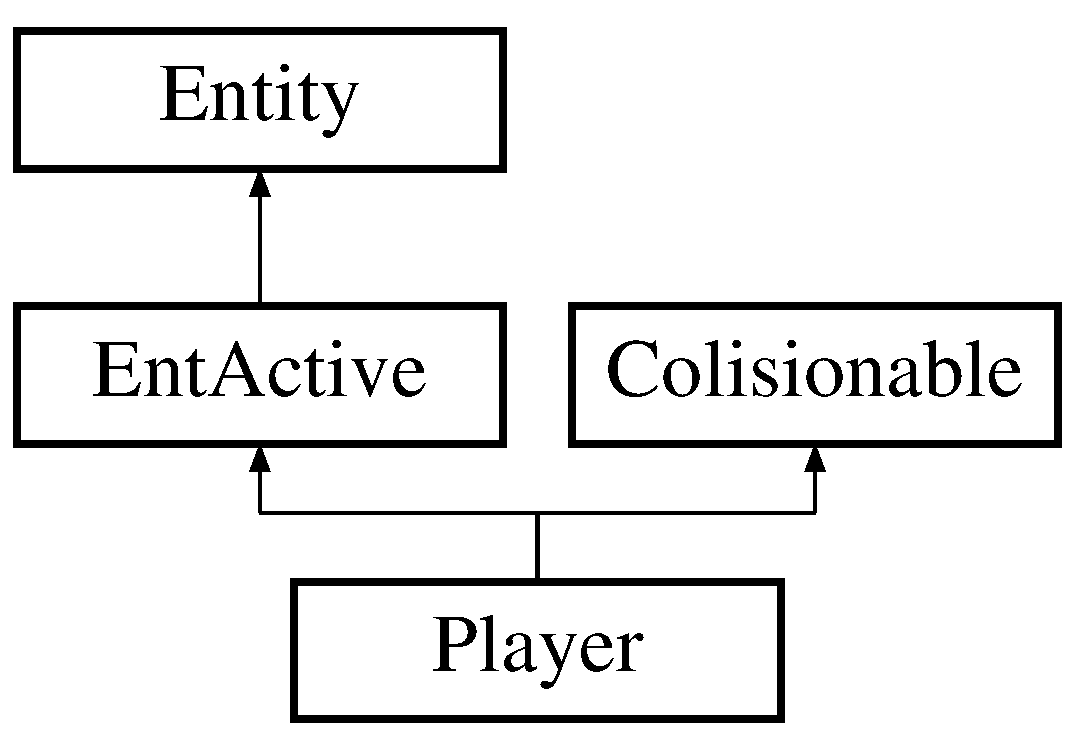
\includegraphics[height=3.000000cm]{classPlayer}
\end{center}
\end{figure}
\subsection*{Métodos públicos}
\begin{DoxyCompactItemize}
\item 
\hypertarget{classPlayer_acddb2634188f14201f7eaa29d8f2611d}{{\bfseries Player} (const sf\-::\-Texture \&tex, bool cen=true)}\label{classPlayer_acddb2634188f14201f7eaa29d8f2611d}

\item 
\hypertarget{classPlayer_a0b67a0b2cbbf4880c35de511fa361dea}{{\bfseries Player} (const sf\-::\-Texture \&tex, const \hyperlink{classVector}{Vector} \&pos, const \hyperlink{classVector}{Vector} \&vel=\hyperlink{classVector}{Vector}(0.f, 0.f), const \hyperlink{classVector}{Vector} \&maxvel=\hyperlink{classVector}{Vector}(600.f, 600.f), bool cen=true)}\label{classPlayer_a0b67a0b2cbbf4880c35de511fa361dea}

\item 
\hypertarget{classPlayer_a3fda0565e6cb6d24c72160e6f88525f2}{{\bfseries Player} (const \hyperlink{classPlayer}{Player} \&orig)}\label{classPlayer_a3fda0565e6cb6d24c72160e6f88525f2}

\item 
\hypertarget{classPlayer_a089deaac2cdf0522d61ebe00647e9054}{virtual const std\-::string {\bfseries Get\-Class\-Name} ()}\label{classPlayer_a089deaac2cdf0522d61ebe00647e9054}

\item 
virtual void \hyperlink{classPlayer_a6fa2109456d203d45b0460fa53ff247b}{Draw} (\hyperlink{classRenderWindow}{Render\-Window} \&window, float inter)
\begin{DoxyCompactList}\small\item\em Realiza un Draw Interpolado. \end{DoxyCompactList}\item 
\hypertarget{classPlayer_ae080f22f3c126845623b043a794175c8}{virtual void \hyperlink{classPlayer_ae080f22f3c126845623b043a794175c8}{Update} (const \hyperlink{classTime}{Time} \&elapsed\-Time)}\label{classPlayer_ae080f22f3c126845623b043a794175c8}

\begin{DoxyCompactList}\small\item\em Realizará un Update de la física, además el propio en las clases hijas. \end{DoxyCompactList}\item 
\hypertarget{classPlayer_a332f6a6235d2cf5f60bd5e8ea11f2b96}{void {\bfseries Add\-Gun} (\hyperlink{classGun}{Gun} $\ast$g)}\label{classPlayer_a332f6a6235d2cf5f60bd5e8ea11f2b96}

\item 
\hypertarget{classPlayer_ade865da0a877ed80544a8980d5bfe6c3}{void {\bfseries Select\-Gun} (int i)}\label{classPlayer_ade865da0a877ed80544a8980d5bfe6c3}

\item 
\hypertarget{classPlayer_a00d075436bc7b9f0e7cfb8f61eadd42b}{\hyperlink{classGun}{Gun} $\ast$ {\bfseries Get\-Selected\-Gun} () const }\label{classPlayer_a00d075436bc7b9f0e7cfb8f61eadd42b}

\item 
\hypertarget{classPlayer_a38b8edc101cf42990dd1ed91c1ae02af}{void {\bfseries Shot} (float x, float y)}\label{classPlayer_a38b8edc101cf42990dd1ed91c1ae02af}

\item 
\hypertarget{classPlayer_adfd1228493c13be267e20fb06aaab45c}{void {\bfseries Do\-Event} (sf\-::\-Keyboard\-::\-Key key, bool is\-Pressed)}\label{classPlayer_adfd1228493c13be267e20fb06aaab45c}

\item 
\hypertarget{classPlayer_abf2ac31c8cd39d8c675d13edf736251f}{void {\bfseries On\-Colision} (Colision\-::\-Type type, const \hyperlink{classRectangle}{Rectangle} \&rec)}\label{classPlayer_abf2ac31c8cd39d8c675d13edf736251f}

\end{DoxyCompactItemize}
\subsection*{Atributos públicos}
\begin{DoxyCompactItemize}
\item 
\hypertarget{classPlayer_ac52a873571f7739cbc506253a3c72660}{std\-::vector$<$ \hyperlink{classGun}{Gun} $\ast$ $>$ $\ast$ {\bfseries guns}}\label{classPlayer_ac52a873571f7739cbc506253a3c72660}

\item 
\hypertarget{classPlayer_a263ff9a2e3d008f3d92013bf9aa3bbb1}{int {\bfseries selected\-Gun}}\label{classPlayer_a263ff9a2e3d008f3d92013bf9aa3bbb1}

\end{DoxyCompactItemize}
\subsection*{Otros miembros heredados}


\subsection{Documentación de las funciones miembro}
\hypertarget{classPlayer_a6fa2109456d203d45b0460fa53ff247b}{\index{Player@{Player}!Draw@{Draw}}
\index{Draw@{Draw}!Player@{Player}}
\subsubsection[{Draw}]{\setlength{\rightskip}{0pt plus 5cm}void Player\-::\-Draw (
\begin{DoxyParamCaption}
\item[{{\bf Render\-Window} \&}]{window, }
\item[{float}]{inter}
\end{DoxyParamCaption}
)\hspace{0.3cm}{\ttfamily [virtual]}}}\label{classPlayer_a6fa2109456d203d45b0460fa53ff247b}


Realiza un Draw Interpolado. 

Dibujado con interpolacion. 

Reimplementado de \hyperlink{classEntActive_a658baff215085c022d8a019269185a66}{Ent\-Active}.



La documentación para esta clase fue generada a partir de los siguientes ficheros\-:\begin{DoxyCompactItemize}
\item 
/home/linuxero/\-Net\-Beans\-Projects/prueba\-\_\-colisiones/\-Clases/Player.\-h\item 
/home/linuxero/\-Net\-Beans\-Projects/prueba\-\_\-colisiones/\-Clases/Player.\-cpp\end{DoxyCompactItemize}

\hypertarget{classRectangle}{\section{Referencia de la Clase Rectangle}
\label{classRectangle}\index{Rectangle@{Rectangle}}
}
\subsection*{Métodos públicos}
\begin{DoxyCompactItemize}
\item 
\hypertarget{classRectangle_a35b73b4806da6084d158cfa0614f6cfb}{{\bfseries Rectangle} (float x, float y, float width, float height, bool from\-Center=false)}\label{classRectangle_a35b73b4806da6084d158cfa0614f6cfb}

\item 
\hypertarget{classRectangle_abd680776a248f74ef546739d9fb16790}{{\bfseries Rectangle} (const sf\-::\-Float\-Rect \&rect)}\label{classRectangle_abd680776a248f74ef546739d9fb16790}

\item 
\hypertarget{classRectangle_aae32c2492c1fe3f1cd89842b09996f53}{{\bfseries Rectangle} (const \hyperlink{classRectangle}{Rectangle} \&orig)}\label{classRectangle_aae32c2492c1fe3f1cd89842b09996f53}

\item 
\hypertarget{classRectangle_a0ad4f750573944a4b4358b2c593699b2}{\hyperlink{classVector}{Vector} {\bfseries Get\-Top\-Left} () const }\label{classRectangle_a0ad4f750573944a4b4358b2c593699b2}

\item 
\hypertarget{classRectangle_af5baf2119946b98ab32b06a7663013b4}{\hyperlink{classVector}{Vector} {\bfseries Get\-Top\-Right} () const }\label{classRectangle_af5baf2119946b98ab32b06a7663013b4}

\item 
\hypertarget{classRectangle_a5c825d557b6d723b81ba91df03e4cc89}{\hyperlink{classVector}{Vector} {\bfseries Get\-Bottom\-Left} () const }\label{classRectangle_a5c825d557b6d723b81ba91df03e4cc89}

\item 
\hypertarget{classRectangle_af4c56ef54727b28f0f692c1920231853}{\hyperlink{classVector}{Vector} {\bfseries Get\-Bottom\-Right} () const }\label{classRectangle_af4c56ef54727b28f0f692c1920231853}

\item 
\hypertarget{classRectangle_aac422a67dc5898711fd7aa58aadb647e}{float {\bfseries Get\-Width} () const }\label{classRectangle_aac422a67dc5898711fd7aa58aadb647e}

\item 
\hypertarget{classRectangle_a3da1c0010c132fab5724d1233d34f4be}{float {\bfseries Get\-Height} () const }\label{classRectangle_a3da1c0010c132fab5724d1233d34f4be}

\item 
\hypertarget{classRectangle_ad78b74643d71995aa186560295a46ab1}{void {\bfseries Set\-X} (float x)}\label{classRectangle_ad78b74643d71995aa186560295a46ab1}

\item 
\hypertarget{classRectangle_a6cbb0d2df0c694f8da3dd29c962347c9}{void {\bfseries Set\-Y} (float y)}\label{classRectangle_a6cbb0d2df0c694f8da3dd29c962347c9}

\item 
\hypertarget{classRectangle_aebfe60964fa3eeb8d8c1077e17fafc2d}{void {\bfseries Set\-Width} (float w)}\label{classRectangle_aebfe60964fa3eeb8d8c1077e17fafc2d}

\item 
\hypertarget{classRectangle_a6b3191ad8cb3f28015628541161a198d}{void {\bfseries Set\-Height} (float h)}\label{classRectangle_a6b3191ad8cb3f28015628541161a198d}

\item 
\hypertarget{classRectangle_ae63b84fe454f93c5ad1f91a7a51cb1fd}{void {\bfseries Set} (float x, float y, float w, float h)}\label{classRectangle_ae63b84fe454f93c5ad1f91a7a51cb1fd}

\item 
\hypertarget{classRectangle_aa13667e689c7f898bea3533a7f240895}{bool {\bfseries Intersects} (const \hyperlink{classRectangle}{Rectangle} \&rec)}\label{classRectangle_aa13667e689c7f898bea3533a7f240895}

\item 
\hypertarget{classRectangle_a8a4a83fe36fc10ff8611be3cf0b62fd9}{bool {\bfseries Is\-Inside} (\hyperlink{classVector}{Vector} \&vec)}\label{classRectangle_a8a4a83fe36fc10ff8611be3cf0b62fd9}

\item 
\hypertarget{classRectangle_a230df1f21614d17998dc70cd7cdd2972}{sf\-::\-Float\-Rect $\ast$ {\bfseries Get\-Rectangle} () const }\label{classRectangle_a230df1f21614d17998dc70cd7cdd2972}

\end{DoxyCompactItemize}
\subsection*{Atributos protegidos}
\begin{DoxyCompactItemize}
\item 
\hypertarget{classRectangle_a36d4b0c079fb5bad16e819b6dd9ae5ad}{sf\-::\-Float\-Rect $\ast$ {\bfseries rectangle}}\label{classRectangle_a36d4b0c079fb5bad16e819b6dd9ae5ad}

\end{DoxyCompactItemize}


La documentación para esta clase fue generada a partir de los siguientes ficheros\-:\begin{DoxyCompactItemize}
\item 
/home/linuxero/\-Net\-Beans\-Projects/prueba\-\_\-colisiones/\-Clases/Rectangle.\-h\item 
/home/linuxero/\-Net\-Beans\-Projects/prueba\-\_\-colisiones/\-Clases/Rectangle.\-cpp\end{DoxyCompactItemize}

\hypertarget{classRenderState}{\section{Referencia de la Clase Render\-State}
\label{classRenderState}\index{Render\-State@{Render\-State}}
}
\subsection*{Métodos públicos}
\begin{DoxyCompactItemize}
\item 
\hypertarget{classRenderState_ad749377bf54064af4921296f7c5c6b5f}{{\bfseries Render\-State} (const \hyperlink{classRenderState}{Render\-State} \&orig)}\label{classRenderState_ad749377bf54064af4921296f7c5c6b5f}

\item 
\hypertarget{classRenderState_a38a5e2a4458a45ce1b77b61b59b02320}{void {\bfseries Draw} (\hyperlink{classRenderWindow}{Render\-Window} \&window, const \hyperlink{classVector}{Vector} \&pos\-Prev, const \hyperlink{classVector}{Vector} \&pos\-New, float interpolation, \hyperlink{classSprite}{Sprite} \&sp)}\label{classRenderState_a38a5e2a4458a45ce1b77b61b59b02320}

\item 
\hypertarget{classRenderState_aaf28ada21e82dae301d41adae6a35efb}{\hyperlink{classVector}{Vector} {\bfseries Get\-Render\-Position} () const }\label{classRenderState_aaf28ada21e82dae301d41adae6a35efb}

\end{DoxyCompactItemize}


La documentación para esta clase fue generada a partir de los siguientes ficheros\-:\begin{DoxyCompactItemize}
\item 
/home/linuxero/\-Net\-Beans\-Projects/prueba\-\_\-colisiones/Render\-State.\-h\item 
/home/linuxero/\-Net\-Beans\-Projects/prueba\-\_\-colisiones/Render\-State.\-cpp\end{DoxyCompactItemize}

\hypertarget{classRenderWindow}{\section{Referencia de la Clase Render\-Window}
\label{classRenderWindow}\index{Render\-Window@{Render\-Window}}
}
\subsection*{Métodos públicos}
\begin{DoxyCompactItemize}
\item 
\hypertarget{classRenderWindow_a76ea49bd4cfa0de2a6d7198c46f5a6ca}{{\bfseries Render\-Window} (int width, int height, const std\-::string titulo, int color=24)}\label{classRenderWindow_a76ea49bd4cfa0de2a6d7198c46f5a6ca}

\item 
\hypertarget{classRenderWindow_aa668645b5f2dd7d6b076fd7c1932d6c2}{{\bfseries Render\-Window} (const \hyperlink{classRenderWindow}{Render\-Window} \&orig)}\label{classRenderWindow_aa668645b5f2dd7d6b076fd7c1932d6c2}

\item 
\hypertarget{classRenderWindow_afae672189b28d791ff08a5728171edad}{void {\bfseries Draw} (\hyperlink{classSprite}{Sprite} \&sp)}\label{classRenderWindow_afae672189b28d791ff08a5728171edad}

\item 
\hypertarget{classRenderWindow_a9e9630d78d3f4a55df91e2d8e565174e}{void {\bfseries Draw} (const sf\-::\-Text \&t)}\label{classRenderWindow_a9e9630d78d3f4a55df91e2d8e565174e}

\item 
\hypertarget{classRenderWindow_a92325866ed95e94d857324e7245d81ac}{void {\bfseries Draw} (const sf\-::\-Rectangle\-Shape \&r)}\label{classRenderWindow_a92325866ed95e94d857324e7245d81ac}

\item 
\hypertarget{classRenderWindow_a0709228a15fcbabf6723d4d829676eb8}{void {\bfseries Clear} (sf\-::\-Color cl)}\label{classRenderWindow_a0709228a15fcbabf6723d4d829676eb8}

\item 
\hypertarget{classRenderWindow_af81e642b35266ce62c465fac374179ce}{void {\bfseries Display} ()}\label{classRenderWindow_af81e642b35266ce62c465fac374179ce}

\item 
\hypertarget{classRenderWindow_a0e9fd523d9888ca17333e50216ba096c}{void {\bfseries Close} ()}\label{classRenderWindow_a0e9fd523d9888ca17333e50216ba096c}

\item 
\hypertarget{classRenderWindow_a52e145a0533dac734b060a4b88d1d880}{bool {\bfseries Is\-Open} ()}\label{classRenderWindow_a52e145a0533dac734b060a4b88d1d880}

\item 
\hypertarget{classRenderWindow_abff1ddc8df26b594595e93bba6ecf742}{void {\bfseries Set\-Vertical\-Sync\-Enabled} (bool v)}\label{classRenderWindow_abff1ddc8df26b594595e93bba6ecf742}

\item 
\hypertarget{classRenderWindow_a97103ac486ade364b0f43f8004e984da}{void {\bfseries Set\-Frame\-Limit} (unsigned int limit)}\label{classRenderWindow_a97103ac486ade364b0f43f8004e984da}

\item 
\hypertarget{classRenderWindow_a83ac01b4e4f8266272fc44f93f2b795e}{bool {\bfseries Poll\-Event} (sf\-::\-Event \&ev)}\label{classRenderWindow_a83ac01b4e4f8266272fc44f93f2b795e}

\end{DoxyCompactItemize}
\subsection*{Atributos públicos}
\begin{DoxyCompactItemize}
\item 
\hypertarget{classRenderWindow_ab908f6f819a6ce504b65de39865b12ff}{int {\bfseries width}}\label{classRenderWindow_ab908f6f819a6ce504b65de39865b12ff}

\item 
\hypertarget{classRenderWindow_a4e309bfa4dc9904ba186c5de405745d2}{int {\bfseries height}}\label{classRenderWindow_a4e309bfa4dc9904ba186c5de405745d2}

\end{DoxyCompactItemize}


La documentación para esta clase fue generada a partir de los siguientes ficheros\-:\begin{DoxyCompactItemize}
\item 
/home/linuxero/\-Net\-Beans\-Projects/prueba\-\_\-colisiones/\-Clases/Render\-Window.\-h\item 
/home/linuxero/\-Net\-Beans\-Projects/prueba\-\_\-colisiones/\-Clases/Render\-Window.\-cpp\end{DoxyCompactItemize}

\hypertarget{classResourceHolder}{\section{Referencia de la plantilla de la Clase Resource\-Holder$<$ Resource, Identifier $>$}
\label{classResourceHolder}\index{Resource\-Holder$<$ Resource, Identifier $>$@{Resource\-Holder$<$ Resource, Identifier $>$}}
}
\subsection*{Métodos públicos}
\begin{DoxyCompactItemize}
\item 
\hypertarget{classResourceHolder_a26b116af6b3c9e607bc3e1d4b2d46f25}{{\bfseries Resource\-Holder} (const \hyperlink{classResourceHolder}{Resource\-Holder} \&orig)}\label{classResourceHolder_a26b116af6b3c9e607bc3e1d4b2d46f25}

\item 
\hypertarget{classResourceHolder_accb6a2b6bd2da503ddfd57b5c0028a16}{void {\bfseries load} (Identifier id, const std\-::string \&filename)}\label{classResourceHolder_accb6a2b6bd2da503ddfd57b5c0028a16}

\item 
\hypertarget{classResourceHolder_ae83a7a88b2b2a74b6143796eb4452110}{{\footnotesize template$<$typename Parameter $>$ }\\void {\bfseries load} (Identifier id, const std\-::string \&filename, const Parameter \&second\-Param)}\label{classResourceHolder_ae83a7a88b2b2a74b6143796eb4452110}

\item 
\hypertarget{classResourceHolder_a6452638a75b6df7ea7d610f204632850}{Resource \& {\bfseries get} (Identifier id)}\label{classResourceHolder_a6452638a75b6df7ea7d610f204632850}

\item 
\hypertarget{classResourceHolder_a9cdb23504de69625ec8405e94a45448f}{const Resource \& {\bfseries get} (Identifier id) const }\label{classResourceHolder_a9cdb23504de69625ec8405e94a45448f}

\end{DoxyCompactItemize}


La documentación para esta clase fue generada a partir de los siguientes ficheros\-:\begin{DoxyCompactItemize}
\item 
/home/linuxero/\-Net\-Beans\-Projects/prueba\-\_\-colisiones/\-Includes/Resource\-Holder.\-hpp\item 
/home/linuxero/\-Net\-Beans\-Projects/prueba\-\_\-colisiones/\-Includes/Resource\-Holder.\-inl\end{DoxyCompactItemize}

\hypertarget{classSingleton}{\section{Referencia de la Clase Singleton}
\label{classSingleton}\index{Singleton@{Singleton}}
}
\subsection*{Métodos públicos estáticos}
\begin{DoxyCompactItemize}
\item 
\hypertarget{classSingleton_a01073bb7481d82d783309be8ba3f51ba}{static \hyperlink{classSingleton}{Singleton} $\ast$ {\bfseries Instance} ()}\label{classSingleton_a01073bb7481d82d783309be8ba3f51ba}

\end{DoxyCompactItemize}
\subsection*{Métodos protegidos}
\begin{DoxyCompactItemize}
\item 
\hypertarget{classSingleton_a52a8e77a0efb8fc0a4650dbea397c676}{{\bfseries Singleton} (const \hyperlink{classSingleton}{Singleton} \&orig)}\label{classSingleton_a52a8e77a0efb8fc0a4650dbea397c676}

\end{DoxyCompactItemize}


La documentación para esta clase fue generada a partir de los siguientes ficheros\-:\begin{DoxyCompactItemize}
\item 
/home/linuxero/\-Net\-Beans\-Projects/prueba\-\_\-colisiones/\-Clases/Singleton.\-h\item 
/home/linuxero/\-Net\-Beans\-Projects/prueba\-\_\-colisiones/\-Clases/Singleton.\-cpp\end{DoxyCompactItemize}

\hypertarget{classSprite}{\section{Referencia de la Clase Sprite}
\label{classSprite}\index{Sprite@{Sprite}}
}
\subsection*{Métodos públicos}
\begin{DoxyCompactItemize}
\item 
\hypertarget{classSprite_a12db2aa93e0945b2c4e7524797dea595}{{\bfseries Sprite} (const sf\-::\-Texture \&tex, bool cen)}\label{classSprite_a12db2aa93e0945b2c4e7524797dea595}

\item 
\hypertarget{classSprite_a6865b4a603a11323d241d311b6be4883}{{\bfseries Sprite} (const \hyperlink{classSprite}{Sprite} \&orig)}\label{classSprite_a6865b4a603a11323d241d311b6be4883}

\item 
\hypertarget{classSprite_a6ae847a4b9dd3c0e4ae5ecbadf4435bb}{bool {\bfseries Is\-Centered} ()}\label{classSprite_a6ae847a4b9dd3c0e4ae5ecbadf4435bb}

\item 
\hypertarget{classSprite_a7ac80cebb5d5f28ab2368dab973c1024}{void {\bfseries Set\-Center} (float x, float y)}\label{classSprite_a7ac80cebb5d5f28ab2368dab973c1024}

\item 
\hypertarget{classSprite_a7e171c2e0fe70f3e4d6292c5751c9e9c}{void \hyperlink{classSprite_a7e171c2e0fe70f3e4d6292c5751c9e9c}{Center} ()}\label{classSprite_a7e171c2e0fe70f3e4d6292c5751c9e9c}

\begin{DoxyCompactList}\small\item\em Centra el origen del \hyperlink{classSprite}{Sprite}. \end{DoxyCompactList}\item 
\hypertarget{classSprite_acd478ec9eae5f31f1a529ff544aeed21}{void {\bfseries Set\-Orientation} (const Transform\-::\-Orientation orient)}\label{classSprite_acd478ec9eae5f31f1a529ff544aeed21}

\item 
\hypertarget{classSprite_a4a7f7ad5b5ab29c7da849e035ae272ca}{Transform\-::\-Orientation {\bfseries Get\-Orientation} () const }\label{classSprite_a4a7f7ad5b5ab29c7da849e035ae272ca}

\item 
\hypertarget{classSprite_ae08c9b370e8311894dd90ab8e83448b3}{void {\bfseries Move} (\hyperlink{classVector}{Vector} \&v)}\label{classSprite_ae08c9b370e8311894dd90ab8e83448b3}

\item 
\hypertarget{classSprite_ae010503cdb7aaf3d9cbe88dfbca1751a}{void {\bfseries Set\-Position} (const \hyperlink{classVector}{Vector} \&v)}\label{classSprite_ae010503cdb7aaf3d9cbe88dfbca1751a}

\item 
\hypertarget{classSprite_ae94877d7364caa68b2c59f07dfaf14b7}{\hyperlink{classVector}{Vector} {\bfseries Get\-Position} () const }\label{classSprite_ae94877d7364caa68b2c59f07dfaf14b7}

\item 
\hypertarget{classSprite_a5a6ed9cc8ffa5da96f938801959feedc}{\hyperlink{classRectangle}{Rectangle} {\bfseries get\-Local\-Bounds} () const }\label{classSprite_a5a6ed9cc8ffa5da96f938801959feedc}

\item 
\hypertarget{classSprite_a62c65aecd9dee6df6cdcd0c27e3f73d4}{\hyperlink{classRectangle}{Rectangle} {\bfseries get\-Global\-Bounds} () const }\label{classSprite_a62c65aecd9dee6df6cdcd0c27e3f73d4}

\end{DoxyCompactItemize}
\subsection*{Atributos públicos}
\begin{DoxyCompactItemize}
\item 
\hypertarget{classSprite_a77eaa813c82468ee00795259391e2c4b}{sf\-::\-Sprite $\ast$ {\bfseries sprite}}\label{classSprite_a77eaa813c82468ee00795259391e2c4b}

\end{DoxyCompactItemize}


La documentación para esta clase fue generada a partir de los siguientes ficheros\-:\begin{DoxyCompactItemize}
\item 
/home/linuxero/\-Net\-Beans\-Projects/prueba\-\_\-colisiones/\-Clases/Sprite.\-h\item 
/home/linuxero/\-Net\-Beans\-Projects/prueba\-\_\-colisiones/\-Clases/Sprite.\-cpp\end{DoxyCompactItemize}

\hypertarget{classStringUtils}{\section{Referencia de la Clase String\-Utils}
\label{classStringUtils}\index{String\-Utils@{String\-Utils}}
}
\subsection*{Métodos públicos estáticos}
\begin{DoxyCompactItemize}
\item 
\hypertarget{classStringUtils_ae3a176c3a0e659c20f028b8287c01c55}{static \hyperlink{classStringUtils}{String\-Utils} $\ast$ {\bfseries Instance} ()}\label{classStringUtils_ae3a176c3a0e659c20f028b8287c01c55}

\item 
\hypertarget{classStringUtils_a6457ea4bd1f0b815c21358abad33d8f5}{static std\-::string {\bfseries Convert\-Bool} (const bool the\-Boolean)}\label{classStringUtils_a6457ea4bd1f0b815c21358abad33d8f5}

\item 
\hypertarget{classStringUtils_af49b24b3ccda9f7594a4c82a534faeb7}{static std\-::string {\bfseries Convert\-Double} (const double the\-Double)}\label{classStringUtils_af49b24b3ccda9f7594a4c82a534faeb7}

\item 
\hypertarget{classStringUtils_a09cf1af81172e632c5b77e3e369af551}{static std\-::string {\bfseries Convert\-Float} (const float the\-Float)}\label{classStringUtils_a09cf1af81172e632c5b77e3e369af551}

\item 
\hypertarget{classStringUtils_acbe48923ece17963f7e405ff8fe8a222}{static std\-::string {\bfseries Convert\-S\-Int} (const short int the\-Number)}\label{classStringUtils_acbe48923ece17963f7e405ff8fe8a222}

\item 
\hypertarget{classStringUtils_a6341cf3fb9a6b0f2cf885674f507e4bd}{static std\-::string {\bfseries Convert\-Int} (const int the\-Number)}\label{classStringUtils_a6341cf3fb9a6b0f2cf885674f507e4bd}

\item 
\hypertarget{classStringUtils_ae77b09c049b7185d7b42e81fcfde8f85}{static std\-::string {\bfseries Convert\-L\-Int} (const long int the\-Number)}\label{classStringUtils_ae77b09c049b7185d7b42e81fcfde8f85}

\item 
\hypertarget{classStringUtils_a655f332e3216417deb4963956c15a002}{static std\-::string {\bfseries Convert\-U\-S\-Int} (const unsigned short int the\-Number)}\label{classStringUtils_a655f332e3216417deb4963956c15a002}

\item 
\hypertarget{classStringUtils_a1473cfb8fbac6242db68850ff6198626}{static std\-::string {\bfseries Convert\-U\-Int} (const unsigned int the\-Number)}\label{classStringUtils_a1473cfb8fbac6242db68850ff6198626}

\item 
\hypertarget{classStringUtils_a714f5a4ca716f81e62e838b42a42de1b}{static std\-::string {\bfseries Convert\-U\-L\-Int} (const unsigned long int the\-Number)}\label{classStringUtils_a714f5a4ca716f81e62e838b42a42de1b}

\item 
\hypertarget{classStringUtils_a696c2867bce6acd98dbf45455c02c711}{static std\-::string {\bfseries Convert\-Color} (const sf\-::\-Color the\-Color)}\label{classStringUtils_a696c2867bce6acd98dbf45455c02c711}

\item 
\hypertarget{classStringUtils_a9dd2d1ab56ae55566850b25a4ea8c8c1}{static std\-::string {\bfseries Convert\-Vector} (const \hyperlink{classVector}{Vector} \&the\-Vector)}\label{classStringUtils_a9dd2d1ab56ae55566850b25a4ea8c8c1}

\item 
\hypertarget{classStringUtils_a1a1611970c8d17f42edd437c87a5be47}{static bool {\bfseries Parse\-Bool} (std\-::string the\-Value)}\label{classStringUtils_a1a1611970c8d17f42edd437c87a5be47}

\item 
\hypertarget{classStringUtils_aa347d57cb232f4d8de8aa2a198b84ca2}{static double {\bfseries Parse\-Double} (const std\-::string the\-Value)}\label{classStringUtils_aa347d57cb232f4d8de8aa2a198b84ca2}

\item 
\hypertarget{classStringUtils_acac584869fae0146720cdbd4b8eb0274}{static float {\bfseries Parse\-Float} (const std\-::string the\-Value)}\label{classStringUtils_acac584869fae0146720cdbd4b8eb0274}

\item 
\hypertarget{classStringUtils_a21def115ad49839722347efb568ca0b3}{static short int {\bfseries Parse\-S\-Int} (const std\-::string the\-Value)}\label{classStringUtils_a21def115ad49839722347efb568ca0b3}

\item 
\hypertarget{classStringUtils_ad6300ed2506a6543aad2ddea10e9c44e}{static int {\bfseries Parse\-Int} (const std\-::string the\-Value)}\label{classStringUtils_ad6300ed2506a6543aad2ddea10e9c44e}

\item 
\hypertarget{classStringUtils_ac073ad28199a96dff714526ab1913051}{static long int {\bfseries Parse\-L\-Int} (const std\-::string the\-Value)}\label{classStringUtils_ac073ad28199a96dff714526ab1913051}

\item 
\hypertarget{classStringUtils_a63c8b524bebf7ae667c248974e4afe68}{static unsigned short int {\bfseries Parse\-U\-S\-Int} (const std\-::string the\-Value)}\label{classStringUtils_a63c8b524bebf7ae667c248974e4afe68}

\item 
\hypertarget{classStringUtils_a416840a91aea78696aa5f13db5c3f61c}{static unsigned int {\bfseries Parse\-U\-Int} (const std\-::string the\-Value)}\label{classStringUtils_a416840a91aea78696aa5f13db5c3f61c}

\item 
\hypertarget{classStringUtils_abdf7501246277f13bcdd02c064df6e29}{static unsigned long int {\bfseries Parse\-U\-L\-Int} (const std\-::string the\-Value)}\label{classStringUtils_abdf7501246277f13bcdd02c064df6e29}

\item 
\hypertarget{classStringUtils_ae1e4e52dfaa87ba8f03d7ee88670fb08}{static sf\-::\-Color {\bfseries Parse\-Color} (const std\-::string the\-Value)}\label{classStringUtils_ae1e4e52dfaa87ba8f03d7ee88670fb08}

\item 
\hypertarget{classStringUtils_a5b6b599bb6b95d193b955fc21480cf8d}{static \hyperlink{classVector}{Vector} {\bfseries Parse\-Vector} (const std\-::string the\-Value)}\label{classStringUtils_a5b6b599bb6b95d193b955fc21480cf8d}

\end{DoxyCompactItemize}


La documentación para esta clase fue generada a partir de los siguientes ficheros\-:\begin{DoxyCompactItemize}
\item 
/home/linuxero/\-Net\-Beans\-Projects/prueba\-\_\-colisiones/\-Clases/String\-Utils.\-h\item 
/home/linuxero/\-Net\-Beans\-Projects/prueba\-\_\-colisiones/\-Clases/String\-Utils.\-cpp\end{DoxyCompactItemize}

\hypertarget{classTime}{\section{Referencia de la Clase Time}
\label{classTime}\index{Time@{Time}}
}
\subsection*{Métodos públicos}
\begin{DoxyCompactItemize}
\item 
\hypertarget{classTime_afa2ac6347fceedd7a10f847504f5fdef}{{\bfseries Time} (float t)}\label{classTime_afa2ac6347fceedd7a10f847504f5fdef}

\item 
\hypertarget{classTime_a36514b10f14cbc5425e37ea16bb1ad5b}{{\bfseries Time} (const \hyperlink{classTime}{Time} \&orig)}\label{classTime_a36514b10f14cbc5425e37ea16bb1ad5b}

\item 
\hypertarget{classTime_a87ed4eafd5b8a63df39589c66a2ef2ca}{float {\bfseries As\-Seconds} () const }\label{classTime_a87ed4eafd5b8a63df39589c66a2ef2ca}

\item 
\hypertarget{classTime_a37f9b2a4905c4a5a8ff577be28b30141}{int32\-\_\-t {\bfseries As\-Milli\-Seconds} () const }\label{classTime_a37f9b2a4905c4a5a8ff577be28b30141}

\item 
\hypertarget{classTime_ac692565c7a6c518c67779b406e9c7557}{void {\bfseries Set\-Seconds} (float sec)}\label{classTime_ac692565c7a6c518c67779b406e9c7557}

\item 
\hypertarget{classTime_a985babec126c51a80db83455ce70b1c2}{\hyperlink{classTime}{Time} \& {\bfseries operator=} (const \hyperlink{classTime}{Time} \&t)}\label{classTime_a985babec126c51a80db83455ce70b1c2}

\item 
\hypertarget{classTime_a375bf61e99fe0055a401df04a2551939}{\hyperlink{classTime}{Time} \& {\bfseries operator+=} (const \hyperlink{classTime}{Time} \&t)}\label{classTime_a375bf61e99fe0055a401df04a2551939}

\item 
\hypertarget{classTime_a91b5ebd30b5fd7950622773e99cfac31}{\hyperlink{classTime}{Time} \& {\bfseries operator-\/=} (const \hyperlink{classTime}{Time} \&t)}\label{classTime_a91b5ebd30b5fd7950622773e99cfac31}

\item 
\hypertarget{classTime_a03b0960f5169ce6fdb1cf53ad8e6cbba}{bool {\bfseries operator$>$} (const \hyperlink{classTime}{Time} \&t)}\label{classTime_a03b0960f5169ce6fdb1cf53ad8e6cbba}

\end{DoxyCompactItemize}
\subsection*{Atributos públicos}
\begin{DoxyCompactItemize}
\item 
\hypertarget{classTime_a8af45df4ac819cbaa57b2fcdc16722d4}{sf\-::\-Time $\ast$ {\bfseries time}}\label{classTime_a8af45df4ac819cbaa57b2fcdc16722d4}

\end{DoxyCompactItemize}


La documentación para esta clase fue generada a partir de los siguientes ficheros\-:\begin{DoxyCompactItemize}
\item 
/home/linuxero/\-Net\-Beans\-Projects/prueba\-\_\-colisiones/\-Clases/Time.\-h\item 
/home/linuxero/\-Net\-Beans\-Projects/prueba\-\_\-colisiones/\-Clases/Time.\-cpp\end{DoxyCompactItemize}

\hypertarget{classVector}{\section{Referencia de la Clase Vector}
\label{classVector}\index{Vector@{Vector}}
}
\subsection*{Métodos públicos}
\begin{DoxyCompactItemize}
\item 
\hypertarget{classVector_a6f80c73b5f18dcf3f8e36065bdc8b9e5}{\hyperlink{classVector_a6f80c73b5f18dcf3f8e36065bdc8b9e5}{Vector} ()}\label{classVector_a6f80c73b5f18dcf3f8e36065bdc8b9e5}

\begin{DoxyCompactList}\small\item\em Este constructor... \end{DoxyCompactList}\item 
\hypertarget{classVector_a7b248851572c39229270f04c3dd192d8}{{\bfseries Vector} (float x, float y)}\label{classVector_a7b248851572c39229270f04c3dd192d8}

\item 
\hypertarget{classVector_a0400ebe778de707c81e56b247d99dcc0}{{\bfseries Vector} (const \hyperlink{classVector}{Vector} \&orig)}\label{classVector_a0400ebe778de707c81e56b247d99dcc0}

\item 
\hypertarget{classVector_a8af2adf29c3264606ae9bde8b30474d3}{float {\bfseries Get\-X} () const }\label{classVector_a8af2adf29c3264606ae9bde8b30474d3}

\item 
\hypertarget{classVector_a1af22bd600a0c05f82492c126ac3c72a}{float {\bfseries Get\-Y} () const }\label{classVector_a1af22bd600a0c05f82492c126ac3c72a}

\item 
\hypertarget{classVector_a54e0ffe36e8115d95738e22eb64b015f}{void {\bfseries Set\-X} (float x)}\label{classVector_a54e0ffe36e8115d95738e22eb64b015f}

\item 
\hypertarget{classVector_a1e1bfb2e0ebcbb70b397fb853093922a}{void {\bfseries Set\-Y} (float y)}\label{classVector_a1e1bfb2e0ebcbb70b397fb853093922a}

\item 
\hypertarget{classVector_ad5d677f0ac46bb6675ab8ee113f4cd1c}{void \hyperlink{classVector_ad5d677f0ac46bb6675ab8ee113f4cd1c}{Set} (float x, float y)}\label{classVector_ad5d677f0ac46bb6675ab8ee113f4cd1c}

\begin{DoxyCompactList}\small\item\em Setea X e Y. \end{DoxyCompactList}\item 
\hypertarget{classVector_afd28980f3852c328db683e49635e318d}{void {\bfseries Set} (\hyperlink{classVector}{Vector} \&v)}\label{classVector_afd28980f3852c328db683e49635e318d}

\item 
\hyperlink{classVector}{Vector} \& \hyperlink{classVector_ae48c467a9f65d60e2f7455aba4ca1239}{operator=} (const \hyperlink{classVector}{Vector} \&v)
\item 
\hypertarget{classVector_ad06a3f604c7d23c532853b52ddb2b23d}{\hyperlink{classVector}{Vector} \& {\bfseries operator+=} (const \hyperlink{classVector}{Vector} \&t)}\label{classVector_ad06a3f604c7d23c532853b52ddb2b23d}

\item 
\hypertarget{classVector_a749ed57358829f920f201745ad040476}{\hyperlink{classVector}{Vector} \& {\bfseries operator-\/=} (const \hyperlink{classVector}{Vector} \&t)}\label{classVector_a749ed57358829f920f201745ad040476}

\item 
\hypertarget{classVector_ab475df273e334d79c16a58933dec45d4}{\hyperlink{classVector}{Vector} \& {\bfseries operator$\ast$=} (const float f)}\label{classVector_ab475df273e334d79c16a58933dec45d4}

\item 
\hypertarget{classVector_aea366e136af0a69b0115aa52e1f67b1e}{\hyperlink{classVector}{Vector} \& {\bfseries operator/=} (const float f)}\label{classVector_aea366e136af0a69b0115aa52e1f67b1e}

\item 
float \hyperlink{classVector_ae6df47f51fec695b3dabcb9a5fd8079c}{Get\-Module} ()
\item 
\hyperlink{classVector}{Vector} \hyperlink{classVector_ae7db6e0671ea63871cdcce0ffad86b86}{Get\-Normalize} ()
\end{DoxyCompactItemize}


\subsection{Documentación de las funciones miembro}
\hypertarget{classVector_ae6df47f51fec695b3dabcb9a5fd8079c}{\index{Vector@{Vector}!Get\-Module@{Get\-Module}}
\index{Get\-Module@{Get\-Module}!Vector@{Vector}}
\subsubsection[{Get\-Module}]{\setlength{\rightskip}{0pt plus 5cm}float Vector\-::\-Get\-Module (
\begin{DoxyParamCaption}
{}
\end{DoxyParamCaption}
)\hspace{0.3cm}{\ttfamily [inline]}}}\label{classVector_ae6df47f51fec695b3dabcb9a5fd8079c}
$<$Calcula el módulo del vector \hypertarget{classVector_ae7db6e0671ea63871cdcce0ffad86b86}{\index{Vector@{Vector}!Get\-Normalize@{Get\-Normalize}}
\index{Get\-Normalize@{Get\-Normalize}!Vector@{Vector}}
\subsubsection[{Get\-Normalize}]{\setlength{\rightskip}{0pt plus 5cm}{\bf Vector} Vector\-::\-Get\-Normalize (
\begin{DoxyParamCaption}
{}
\end{DoxyParamCaption}
)\hspace{0.3cm}{\ttfamily [inline]}}}\label{classVector_ae7db6e0671ea63871cdcce0ffad86b86}
$<$Normaliza un vector \hypertarget{classVector_ae48c467a9f65d60e2f7455aba4ca1239}{\index{Vector@{Vector}!operator=@{operator=}}
\index{operator=@{operator=}!Vector@{Vector}}
\subsubsection[{operator=}]{\setlength{\rightskip}{0pt plus 5cm}{\bf Vector} \& Vector\-::operator= (
\begin{DoxyParamCaption}
\item[{const {\bf Vector} \&}]{v}
\end{DoxyParamCaption}
)}}\label{classVector_ae48c467a9f65d60e2f7455aba4ca1239}
Esta función Suma X e Y al vector 
\begin{DoxyParams}{Parámetros}
{\em x} & posicion en el eje X \\
\hline
{\em y} & posicion en el eje Y \\
\hline
\end{DoxyParams}
\begin{DoxyReturn}{Devuelve}
No devuelve nada 
\end{DoxyReturn}


La documentación para esta clase fue generada a partir de los siguientes ficheros\-:\begin{DoxyCompactItemize}
\item 
/home/linuxero/\-Net\-Beans\-Projects/prueba\-\_\-colisiones/\-Clases/Vector.\-h\item 
/home/linuxero/\-Net\-Beans\-Projects/prueba\-\_\-colisiones/\-Clases/Vector.\-cpp\end{DoxyCompactItemize}

\hypertarget{classWorld}{\section{Referencia de la Clase World}
\label{classWorld}\index{World@{World}}
}
\subsection*{Métodos públicos}
\begin{DoxyCompactItemize}
\item 
\hypertarget{classWorld_a8f79652f07f99fa41b3db357c4efb895}{void {\bfseries Init} ()}\label{classWorld_a8f79652f07f99fa41b3db357c4efb895}

\item 
\hypertarget{classWorld_acea6eb85cbad062ded1e62193496e9f5}{void {\bfseries Run} ()}\label{classWorld_acea6eb85cbad062ded1e62193496e9f5}

\item 
\hypertarget{classWorld_add9920638985c1c96f2c4616db993ec8}{void {\bfseries Update} (const \hyperlink{classTime}{Time} \&time\-Elapsed)}\label{classWorld_add9920638985c1c96f2c4616db993ec8}

\item 
\hypertarget{classWorld_a4623e37c9b4df02ab156cb185d239df8}{void {\bfseries Render} (float interp)}\label{classWorld_a4623e37c9b4df02ab156cb185d239df8}

\item 
\hypertarget{classWorld_a9b75a4c608052f44f6a712e3d4533169}{void \hyperlink{classWorld_a9b75a4c608052f44f6a712e3d4533169}{Process\-Events} ()}\label{classWorld_a9b75a4c608052f44f6a712e3d4533169}

\begin{DoxyCompactList}\small\item\em !!!!!!!!!!!!!!! Esto lo haría el gestor de eventos, pero se hará mas adelante \end{DoxyCompactList}\item 
\hypertarget{classWorld_a30d86a6a40eef22070409ba0f2c88e70}{void {\bfseries Callback} (sf\-::\-Keyboard\-::\-Key key, bool is\-Pressed)}\label{classWorld_a30d86a6a40eef22070409ba0f2c88e70}

\item 
\hypertarget{classWorld_a110e10c5169c9edeabc1112e1e6e1a77}{void {\bfseries Add\-Static\-Entity} (\hyperlink{classEntPassive}{Ent\-Passive} $\ast$ent)}\label{classWorld_a110e10c5169c9edeabc1112e1e6e1a77}

\item 
\hypertarget{classWorld_a2eb1f61d62b1855a5640b5ccc7b61e90}{void {\bfseries Add\-Active\-Entity} (\hyperlink{classEntActive}{Ent\-Active} $\ast$ent)}\label{classWorld_a2eb1f61d62b1855a5640b5ccc7b61e90}

\item 
\hypertarget{classWorld_a7e82762690a692ef7eb3c0792a28b7ec}{void {\bfseries Add\-Colisionable\-Entity} (\hyperlink{classColisionable}{Colisionable} $\ast$ent)}\label{classWorld_a7e82762690a692ef7eb3c0792a28b7ec}

\end{DoxyCompactItemize}
\subsection*{Métodos públicos estáticos}
\begin{DoxyCompactItemize}
\item 
\hypertarget{classWorld_a1881ce92c156c24c864a8fd079be20c2}{static \hyperlink{classWorld}{World} $\ast$ {\bfseries Instance} ()}\label{classWorld_a1881ce92c156c24c864a8fd079be20c2}

\end{DoxyCompactItemize}
\subsection*{Atributos públicos}
\begin{DoxyCompactItemize}
\item 
\hypertarget{classWorld_afaed9604e36a6a5a562da7294af39be2}{\hyperlink{classLevel}{Level} $\ast$ {\bfseries level}}\label{classWorld_afaed9604e36a6a5a562da7294af39be2}

\item 
\hypertarget{classWorld_addf54f12f3a1e9c8f120265bafa3474e}{\hyperlink{classPlayer}{Player} $\ast$ {\bfseries player}}\label{classWorld_addf54f12f3a1e9c8f120265bafa3474e}

\item 
\hypertarget{classWorld_af6e54a7d400b0e589cfaad872af0f1b6}{\hyperlink{classResourceHolder}{Resource\-Holder}$<$ sf\-::\-Texture, \\*
std\-::string $>$ $\ast$ {\bfseries cont\-Textures}}\label{classWorld_af6e54a7d400b0e589cfaad872af0f1b6}

\item 
\hypertarget{classWorld_a2767a70043e32c81784b3deb96f0c8e5}{\hyperlink{classResourceHolder}{Resource\-Holder}$<$ sf\-::\-Font, \\*
std\-::string $>$ $\ast$ {\bfseries cont\-Fonts}}\label{classWorld_a2767a70043e32c81784b3deb96f0c8e5}

\item 
\hypertarget{classWorld_a7365975cf93c7a9b4868c53c4ac189a2}{std\-::vector$<$ sf\-::\-Rectangle\-Shape $>$ {\bfseries v\-Rectangle\-Shape}}\label{classWorld_a7365975cf93c7a9b4868c53c4ac189a2}

\item 
\hypertarget{classWorld_a7c5f3199bedf69881b6fc5957fc2d1f9}{std\-::vector$<$ \hyperlink{classBullet}{Bullet} $\ast$ $>$ $\ast$ {\bfseries v\-Bullets}}\label{classWorld_a7c5f3199bedf69881b6fc5957fc2d1f9}

\end{DoxyCompactItemize}


La documentación para esta clase fue generada a partir de los siguientes ficheros\-:\begin{DoxyCompactItemize}
\item 
/home/linuxero/\-Net\-Beans\-Projects/prueba\-\_\-colisiones/\-Clases/World.\-h\item 
/home/linuxero/\-Net\-Beans\-Projects/prueba\-\_\-colisiones/\-Clases/World.\-cpp\end{DoxyCompactItemize}

%--- End generated contents ---

% Index
\newpage
\phantomsection
\addcontentsline{toc}{chapter}{Índice}
\printindex

\end{document}
